\chapter{Tail-Anchored Protein Datasets}
\sloppy

\section{Abstract}

\section{Introduction}

\gls{ta} proteins are defined by their single carboxy-terminal~\gls{tmh} with a cytosolic facing amino-terminus and are a topologically distinct class of intracellular proteins.
The integration of \gls{ta} proteins into the membrane is post-translational rather than co-translational; the ribosome is not in complex with the membrane insertion machinery.
~\gls{ta} proteins are involved in a range of key cellular functions such as translocation \cite{Osborne2005} such as Sec61$\beta$ and Sec61$\gamma$ as well as the Bcl-2 apoptotic protein family  \cite{Hockenbery1990}.
Additionally, within the~\gls{ta} class of proteins are a set of vesicle fusion proteins called~\gls{snare} proteins \cite{Ungar2003}, which     contain typically hydrophobic \gls{tmh}s \cite{Kalbfleisch2007}.
The idea that \gls{snare} proteins are modular and capable of spontaneous insertion has significant implications for both biomedical application in liposome\--based drug delivery and can aid future research for testing complex biological molecular networks~\cite{Allen2013, Nordlund2014}.

The \gls{ta} protein's \gls{tmh} is unusual in that it is both the anchor and the targeting factor for the \gls{er} \cite{Kutay1993}.
Furthermore, the hydrophobicity appears to be a determining factor in the delivery pathway that~\gls{ta} proteins use for insertion~\cite{Rabu2008, Rabu2009}, for which there is evidence demonstrating that are several mechanisms of translocation~\cite{Rabu2009, Johnson2013}(Figure \ref{fig:biogenesis-overview}).
%Alternative mechanisms (Kutay et al., 1995; Nyathi et al., 2013; Chartron et al., 2012)

\begin{sidewaysfigure}
\centering
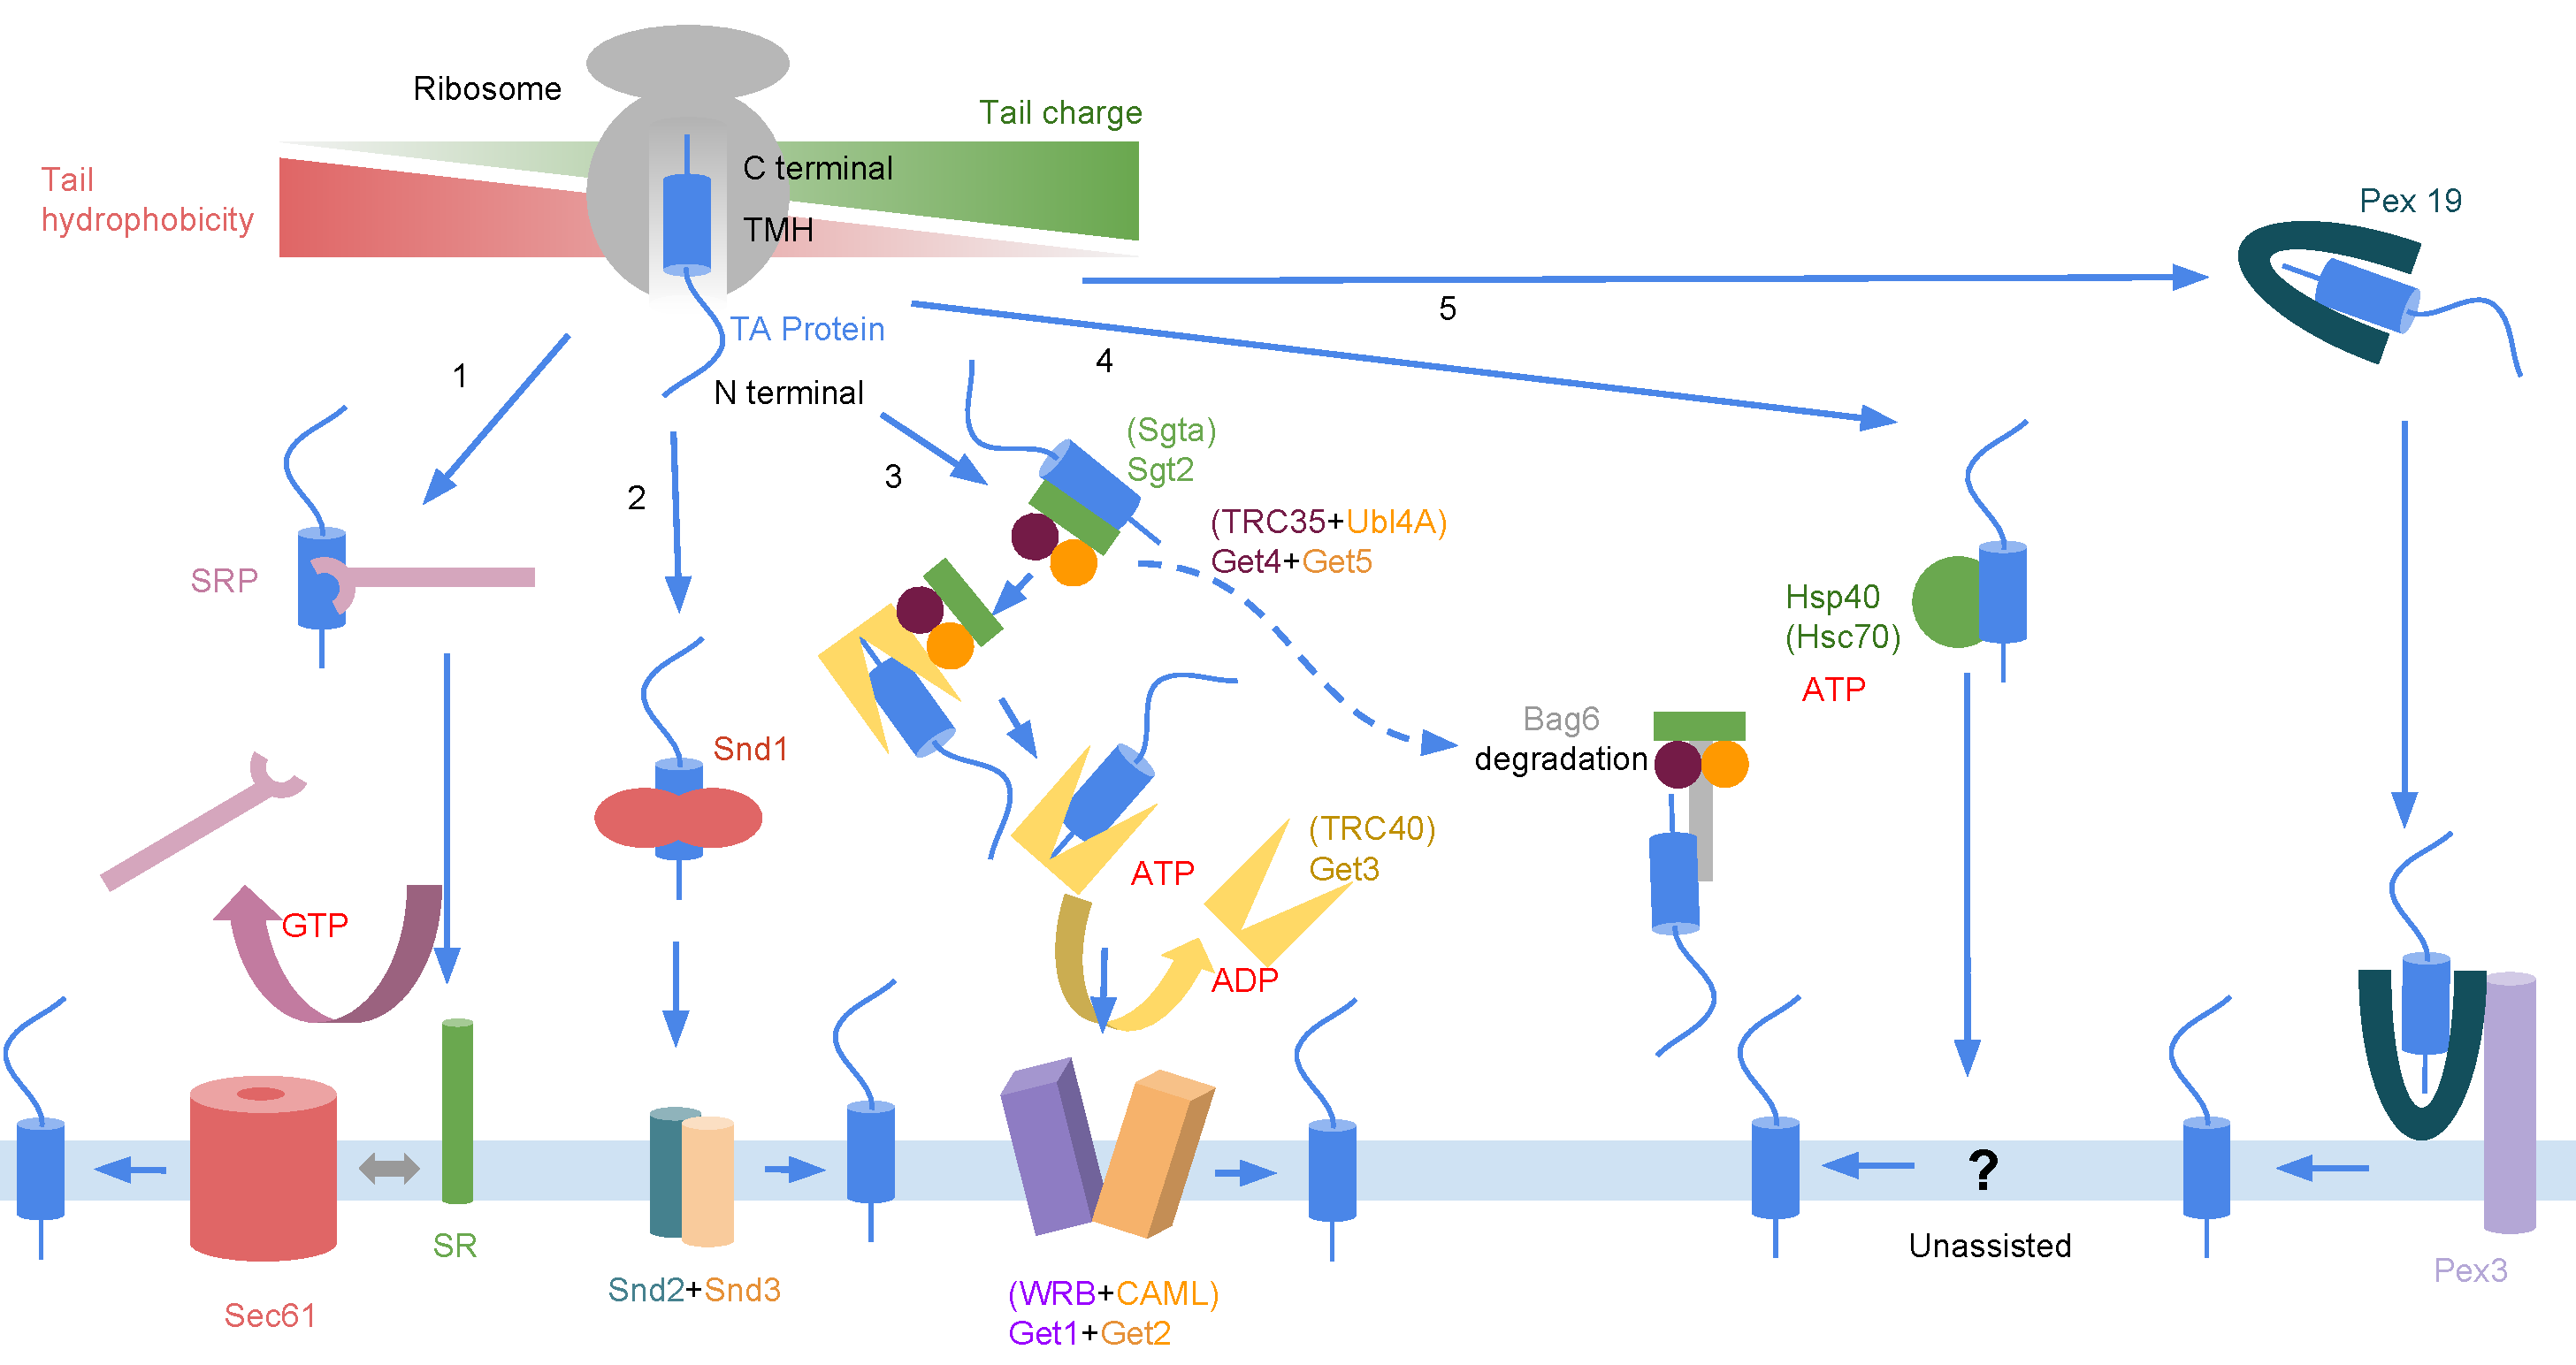
\includegraphics[width=1\textwidth]{TA_chapter/biogenesis-overview}
        \captionof{figure}[An overview of the biogenesis of tail-anchored proteins.]{\textbf{An overview of the biogenesis of tail-anchored proteins.}
        (1) \gls{srp} and Sec61 of the co-translational insertion mechanism have been shown to be able to integrate \gls{ta} proteins.
        (2) In yeast, a novel mechanism was identified in which Snd1 binds to the folded \gls{ta} protein and delivers it to the membrane\--bound Snd2 and Snd3 complex.
        (3) The intensively studied Get (yeast) or TRC40 (mammalian) pathway can target either for membrane integration or degradation of the \gls{ta} protein.
        (4) A handful of \gls{ta} proteins with relatively polar \gls{tmh} regions have been observed spontaneously integrating into the membrane using Hsp40 and Hsc70 as chaperones.
        This system may be employed for mitochondrial localisation.
        (5) Peroxisomal proteins with an abundance of charge in the tail region are chaperoned by Pex19 into association with the membrane\--bound Pex3.
}

\label{fig:biogenesis-overview}
\end{sidewaysfigure}

\gls{ta} proteins have several pathways for biogenesis in the~\gls{er} membrane.
\gls{ta} proteins were originally thought to be inserted into the membrane via different machinery than the co-translational machinery, but unexpectedly \gls{srp} was found to be a factor for post-translational targeting confirmed by both cross-linking studies \cite{Abell2004} and an \textit{in vitro} pull-down experiment \cite{Leznicki2010}.
\gls{srp} would deliver the \gls{ta} protein to the membrane\--bound \gls{sr} in association with a highly conserved Sec translocon.
Further cross-linking experiments suggested Sec61 is also involved during \gls{ta} protein membrane insertion \cite{Abell2003}.
Previous studies had shown the Sec61 translocon is not necessary for \gls{ta} protein membrane integration by biochemical reconstitution experiments \cite{Kutay1993} and conditional mutants in yeast \cite{Steel2002, Yabal2003}. %What kind of mutants?
Nevertheless, this suggests the possibility of at least one insertion mechanism that is related to the co-translational method of insertion (Figure \ref{fig:biogenesis-overview} (1)).

A second possibly redundant system is also known to be involved in \gls{ta} protein biogenesis and is referred to as the TRC40 (also known as Asna1) pathway in mammals (Figure \ref{fig:biogenesis-overview} (3)).
A conserved homologue was found in \textit{Saccharomyces cerevisiae}, Get3 \cite{Schuldiner2008}, and in yeast, this mechanism is generally referred to as the Get pathway.
Unlike co-translational insertion, the post-translational proteins do not couple with the ribosome, so the \gls{ta} protein must be exposed to the cytosolic environment for at least some time \cite{Guna2018}.
At some point after the \gls{ta} protein emerges from the ribosomal exit tunnel, the \gls{ta} protein \gls{tmh} associates with Sgt2.
An \textit{in vitro} assay revealed that Sgt2 associates with Get5  \cite{Wang2010} as part of a dimerised Get4 and Get5 complex (two copies of each)\cite{Chang2010, Chang2012, Chartron2010, Chartron2012}.
At this point Sgt2 either associates with preferential Get3 which targets the \gls{ta} protein for \gls{er} membrane biogenesis or if there are excess \gls{ta} proteins Sgt2 also associates with Bag6 which targets the \gls{ta} protein for degradation \cite{Shao2017}.
This ``race'' between Bag6 and Get3 ensures a level of quality control within the system.
Assuming the \gls{ta} protein is not targetted for degradation, Get3 associates first with this complex via an interaction with the N-terminal of Get4 \cite{Wang2010}.
A dimerised ADP-bound Get3 \cite{Mateja2009, Hu2009, Bozkurt2009, Suloway2009, Yamagata2010} (TRC40) associates with and shields the C-terminal region of the \gls{ta} protein \cite{Stefanovic2007, Schuldiner2008, Favaloro2008}.
This shielding may be especially important since Get3 is involved in the folding of any nascent \gls{ta} proteins, which would be an unviable hydrophobic in the cytosol \cite{Jonikas2009}.
Fluorescence studies revealed that tagged Get3 appears at both the cytosol and the \gls{er} membrane so apparently shuttles the \gls{ta} protein between the transmembrane complex of Get1 and Get 2 (WRB and CAML in mammalian cells), that contains cytosolic domains that receive Get3, and Get4 Get5 Sgt2 complex \cite{Huh2003, Zalisko2017}.
Yet it is an interesting note that a single molecule fluorescence study revealed that the minimum machinery required for \gls{ta} protein insertion from this system is a Get1 and Get2 heterodimer \cite{Zalisko2017}.

Redundancy of the Get/TRC40 pathway and \gls{srp} pathway may be explained in part by a novel \gls{srp} and Get independent pathway.
This pathway utilises the Snd protein pathway and was discovered in yeast \cite{Aviram2016} (Figure \ref{fig:biogenesis-overview} (2)).
Snd1 binds to the \gls{ta} protein after it exits the ribosome and delivers it to the Snd2 and Snd3 membrane\--bound complex which integrates the \gls{ta} protein into the membrane.

In the absence of the mitochondrial TIM-TOM insertion machinery and Get machinery, Hsp40 and Hsc70 chaperones along with ATP are also sufficient for enough biogenesis of \gls{ta} proteins for viable cell growth \cite{Rabu2008, Rabu2009, Ngosuwan2003, Colombo2009, Kemper2008, Meineke2008, Setoguchi2006}.
In biological systems, this is possibly used for mitochondrial delivery \cite{Kemper2008} (Figure \ref{fig:biogenesis-overview} (4)).
Chimeric synaptobrevin, one of the first identified~ \gls{snare} proteins, is capable of this spontaneous insertion if the tail anchor domain is replaced by the~\gls{tm} domains belonging to a protein of known spontaneously inserting domains \cite{Nordlund2014}.
Molecular dynamics simulations showed that direct insertion \gls{tmh}s thermodynamically mimics the energies of \gls{tmh}s integrated by the translocon \cite{Ulmschneider2014} so in theory, no integration machinery is strictly necessary if the \gls{tmh} can ``correctly'' interact with the membrane interface.
Further, it was revealed that scrambling the \gls{tmh} sequence, but maintaining hydrophobicity, reduced the insertion potential of spontaneously inserting \gls{tmh}s \cite{Brambillasca2006}.
This phenomenon cannot, therefore, be explained entirely by the marginal hydrophobicity of the \gls{tmh}.

The few peroxisomal \gls{ta} proteins first associate with Pex19 which forms a complex with the membrane\--anchored Pex3 protein from which the \gls{ta} protein is integrated into the membrane \cite{Chen2014, Yagita2013, Costello2017}(Figure \ref{fig:biogenesis-overview} (5)).

Given a ``choice'', it is speculated that hydrophobicity determines the integration pathway since Sec61$\beta$ has a hydrophobic \gls{tmh} and is targetted via the \gls{srp} pathway, whereas marginally hydrophobic \gls{ta} proteins like cytochrome b5 and PTP1b can spontaneously insert \textit{in vitro} and biologically only rely on Hsp70 and Hsc40.
Altering the hydrophobicity, at least in the case of the spontaneously inserting PTP1b, also determinates the localisation of the \gls{ta} protein to either the mitochondrial membrane or the \gls{er} membrane, or rather a more hydrophobic \gls{ta} protein \gls{tmh} is less likely to localise to the mitochondrial membrane \cite{Fueller2015}.
Broader analysis has shown that hydrophobicity \cite{White1999} stratified by TM tendency score \cite{Zhao2006} can distinguish between the \gls{er} and mitochondrial localised \gls{ta} proteins \cite{Guna2018}.
However, the tremendous diversity and known biogenesis redundancy of these proteins may mean that no single factor applied en masse may be able to distinguish the \gls{tmh} recognition factors and investigation into this area is becoming increasingly complex \cite{Guna2018}.

By regenerating a list of likely \gls{tmh}s \cite{Kalbfleisch2007} and using a manually curated list of \gls{ta} proteins \cite{TheUniProtConsortium2014}, this investigation aims to find relationships between biochemical factors and a disposition to a certain insertion mechanism and terminal localisations.
Here, we also present evidence for a conserved polar strip along the spontaneously inserting \gls{ta} protein \gls{tmh}s, which may be the key to the initial interaction of these \gls{tmh}s with the membrane interface.

\section{Methods}

\subsection{Building a List of Tail-Anchors}
Steps carried out by Kalbfleisch \textit{et al.} (Traffic 8: 1687\-1694) to generate a list of all \gls{ta} proteins in the human proteome ~\cite{Kalbfleisch2007}, were recreated using up to date tools and applied to other model representitive species.
Whilst their study focused on the human proteome, here we take into account the entire TrEMBL and SwissProt database and then stratify the datasets by the organism at the end of the pipeline (Figure \ref{fig:dataset-overview}).

\begin{figure}[!ht]
\centering
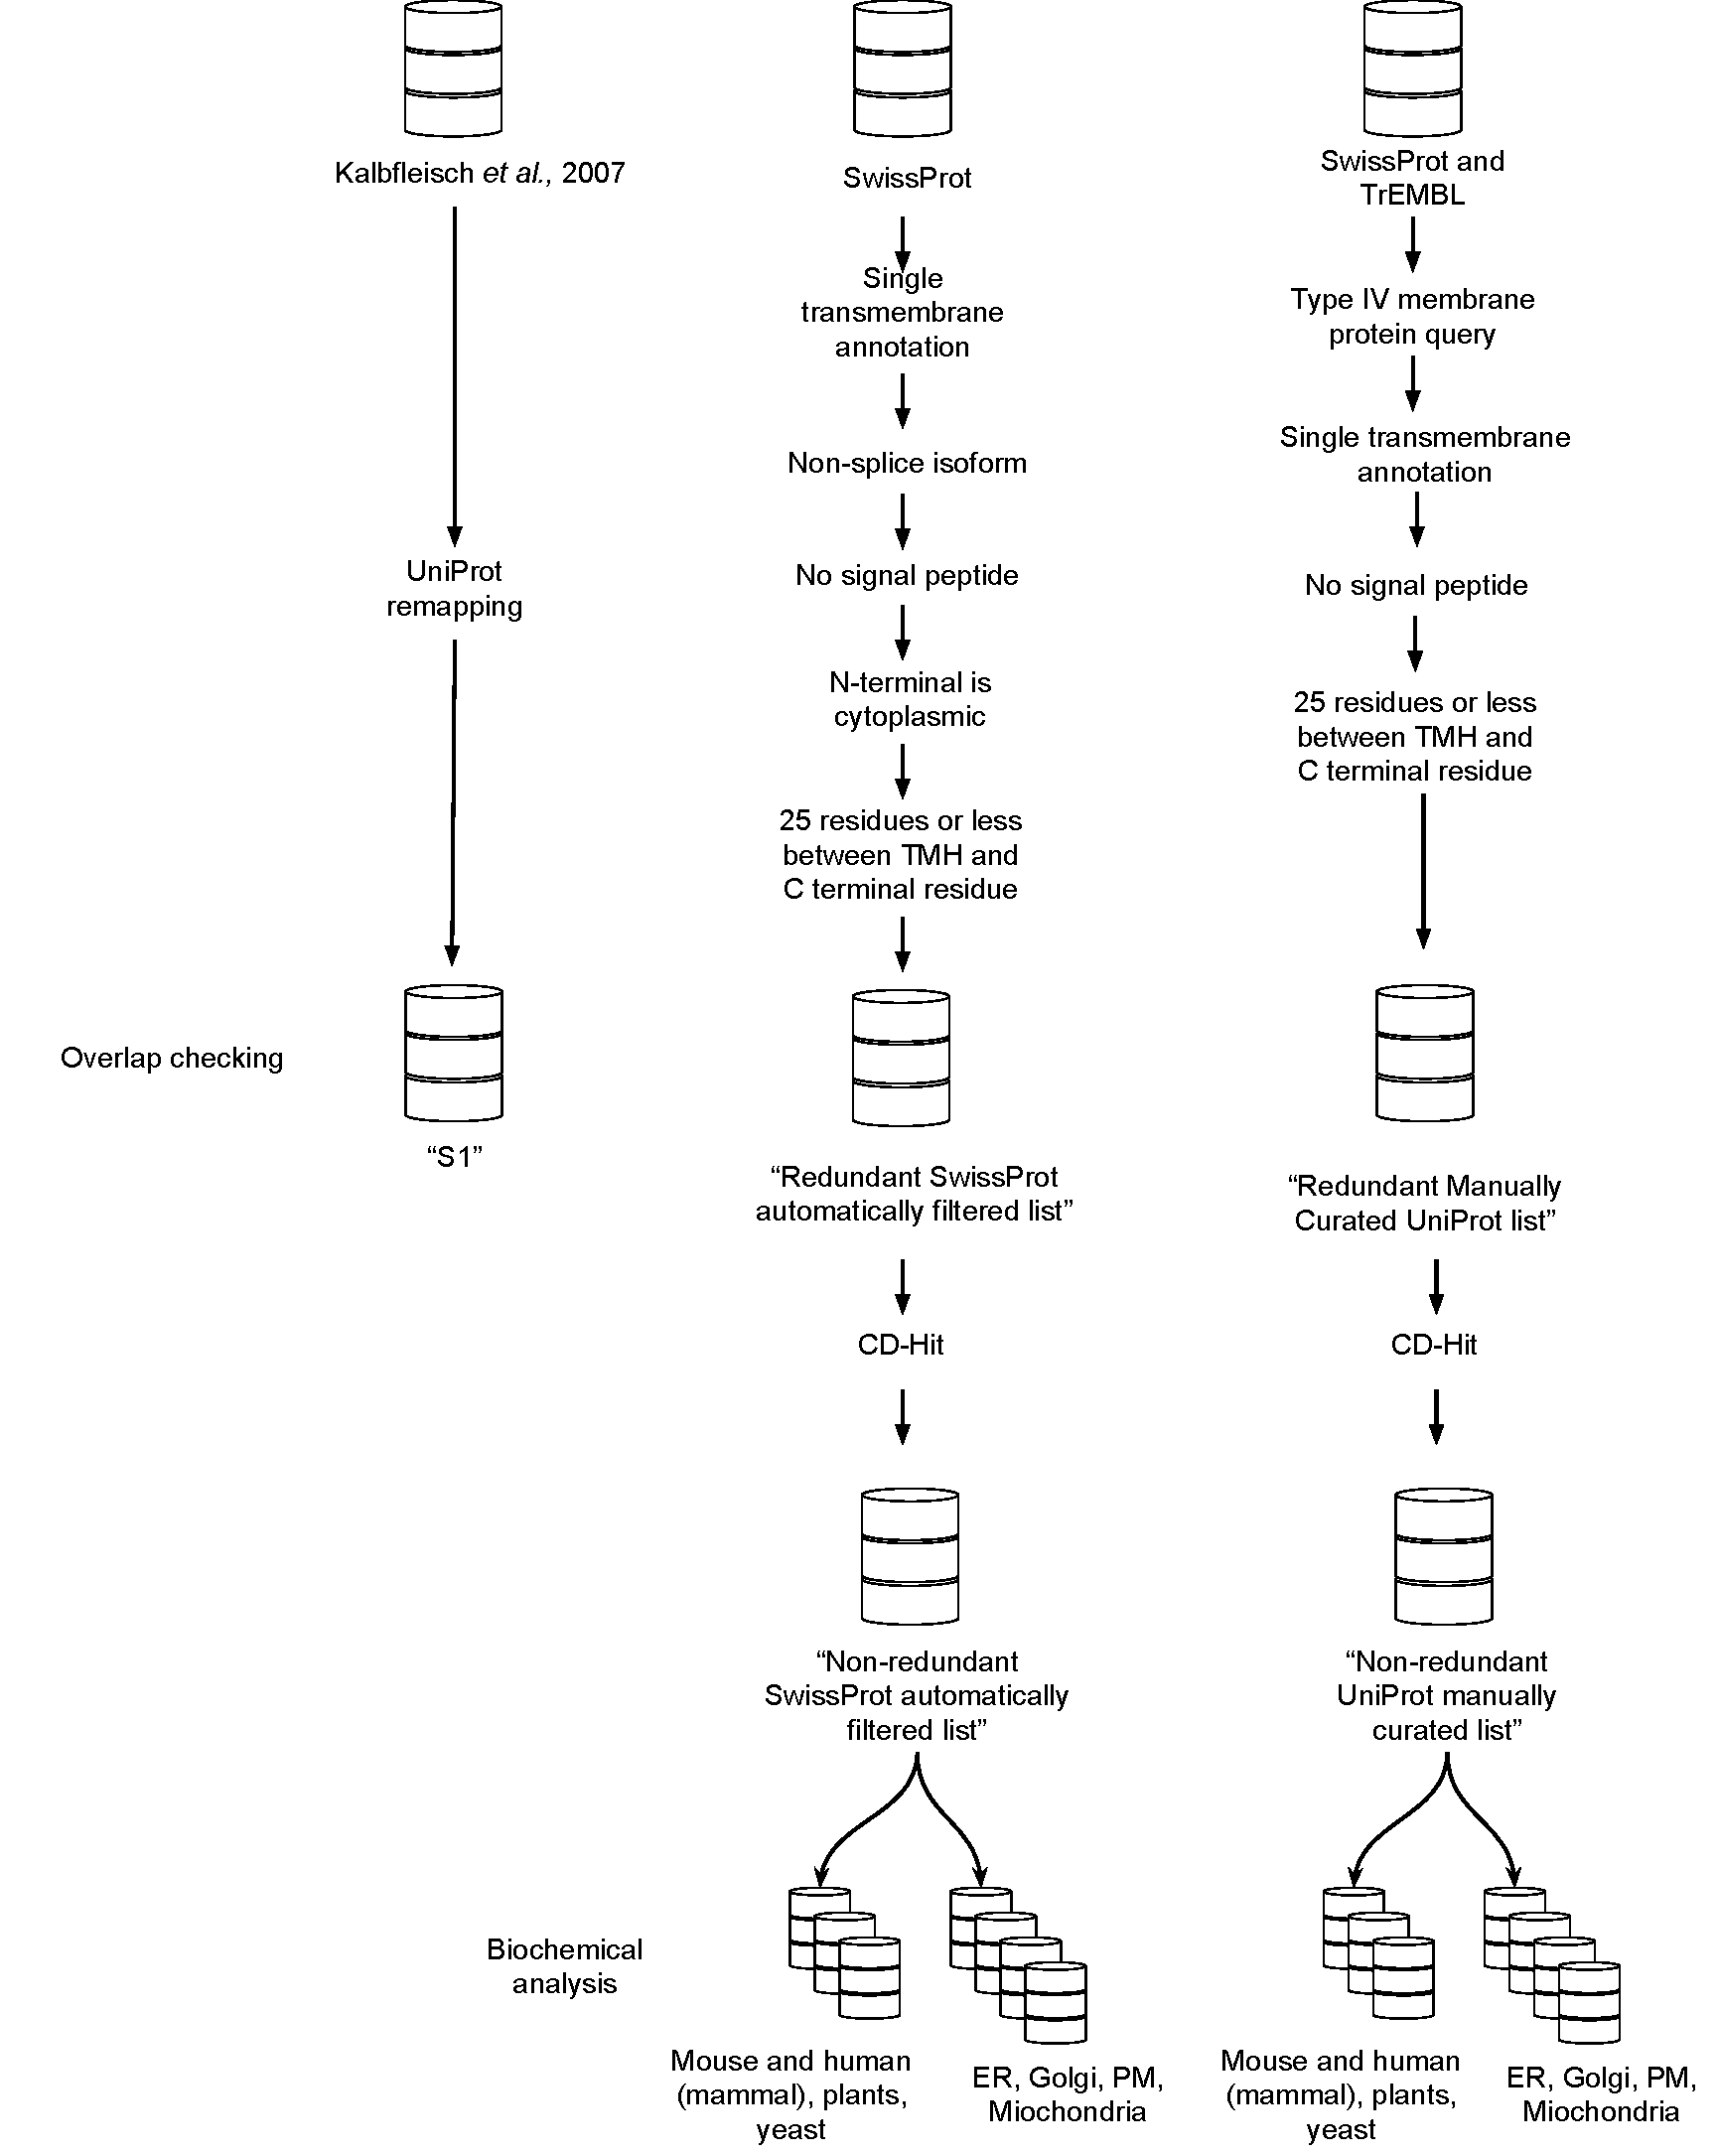
\includegraphics[width=1\textwidth]{TA_chapter/dataset-overview}
        \captionof{figure}[The sources, methods, and filters applied to the sequences in the datasets.]{\textbf{The sources, methods, and filters applied to the sequences in the datasets.}
        From top to bottom are the sources of the sequences and the filters and methods applied to each of the datasets of sequences. The database symbol is used to denote when the dataset was used to capture results and is available as supplementary material. For the dataset size and more information, see the methods section text.
}

\label{fig:dataset-overview}
\end{figure}

\subsubsection{SwissProt Tail Anchored Dataset According to Filters}
There were 557012 protein records downloaded from SwissProt via UniProt~\cite{TheUniProtConsortium2014} (downloaded 24--04--2018).
106149~\gls{tmh}s (\url{TRANSMEM} annotation) were found between 76953 records (\url{annotation:(type:transmem) AND reviewed:no}).
This keyword is contained in a record according to either experimental evidence~\cite{TheUniProtConsortium2014} or a conservative meta-analysis of~\gls{tmh} prediction using TMHMM~\cite{Krogh2001}, Memsat~\cite{Jones2007}, Phobius~\cite{Kall2004,Kall2007} and the hydrophobic moment plot method of Eisenberg and co-workers~\cite{Eisenberg1984}.
11141 of those records had only a single~\gls{tmh}.
11110 of those~\gls{tmh}s were within the length thresholds of 16 to 30 residues (None of those had the annotation for splice isoforms according to \url{NON_TER} annotation).
5548 of those had had no~\gls{sp} annotation (\url{SIGNAL}).
4332 of those had annotation (based on \url{TOPO_DOM} annotation) that the N terminal was cytoplasmic.
615 of those had the~\gls{tmh} within 25 residues of the C terminal, the same threshold used by Kalbfleisch \textit{et al.,}~\cite{Kalbfleisch2007}.
Running CD-Hit 4.5.3 on the WebMGA web-server~\cite{Huang2010, Wu2011} at 90\% identical sequence at 90\% coverage thresholds resulted in 443 representative proteins.
This threshold was chosen as a compromise between avoiding over-representation of a certain protein and maintaining a viable sample size.

From this representative list, 46 were Archaeal, 66 were bacterial, and 320 were eukaryotic and 11 came from dsDNA viruses.
When counting proteomes with greater than 20 records, 49 belonged to the \textit{A. thaliana} proteome, 48 to Mouse, 46 to the human proteome, 24 to \textit{S.cerevisiae}. %19 from RAT!

65 were annotated under the mitochondrion location (query \url{locations:(location:"Mitochondrion [SL-0173]")}), 157 in the \gls{pm} (query \url{locations:(location:"Cell membrane [SL-0039]")}, 82 in the Golgi (query \url{locations:(location:"Golgi apparatus [SL-0132]")}), and 98 in the \gls{er} (query \url{locations:(location:"Endoplasmic reticulum [SL-0095]"}).
Only 16 records were found for the peroxisome (query \url{locations:(location:"Endoplasmic reticulum [SL-0204]"}) which is not high enough a sample size for accurate statistical analysis.


\subsubsection{TrEMBL Tail Anchored Dataset According to Filters}
111425234 records were stored in the TrEMBL database at the time of download (downloaded 25--04--2018).
22107826 of those contained \url{TRANSMEM} annotation (\url{annotation:(type:transmem) AND reviewed:no}).
18053 of these were single\--pass proteins.
All of these were within the length restrictions of between 16 and 35 residues for the \gls{tmh} region.
17973 of those did not contain a signal sequence when looking for \url{SIGNAL} annotation.
5157 of those contained a cytoplasmically located N terminal according to \url{TOPO_DOM} annotation.
155 records had a~\gls{tmh} within 25 residues of the C terminal residue.
When considering which species these records come from, no more than 1 record belonged to any given species.
To avoid representing a well-annotated SwissProt record that includes species annotation by a poorly annotated TrEMBL record without species annotation, these TrEMBL records were omitted from the sequence redundancy protocol and further analysis.

\subsubsection{UniProt Curated List}
A query for \url{locations:(location:"Single\--pass type IV membrane protein [SL-9908]")} was used in UniProt which returned 2633 UniProtKB IDs; 463 SwissProt results and 2170 TrEMBL results.
Type IV anchors are sometimes split into two topological groups; A (A cytosolic facing N terminal domain) and B (The N terminal is targeted to the lumen), however, the UniProt nomenclature is strictly N terminal being cytosolic.
This manually created list contained some \gls{ta} proteins that didn't exactly fit the generally accepted definition of a \gls{ta} protein and were excluded from further analysis.
These could be examples of misannotation in the databases, or exceptional \gls{ta} proteins that behave as post-translationally inserted \gls{ta} proteins despite not matching the exact criteria.
101 exceeded the \gls{ta} length restrictions of 25 residues between the \gls{tmh} and the terminal residue.
8 contained annotation for \url{SIGNAL}, indicating an \gls{sp}, inconsistent with the \gls{ta} protein definition.
20 were multipass proteins.
A full list of which records exceeded these limits and by how much is included in the supplementary files.
Running these records through CD-HIT at 90\% redundancy yielded 956 clusters; 269 SwissProt records and 687 TrEMBL records~\cite{Huang2010, Wu2011}.
No further filters were applied to this list.
Proteomes represented by more than 20 records include \textit{A. thaliana} (53 records), Humans (30), Mouse (30), and \textit{S. cerevisiae} (27). % and 20 to Rat.

426 were annotated under the mitochondrion location (query \url{locations:(location:"Mitochondrion [SL-0173]")}) 47 from SwissProt and 379 automatically assigned in TrEMBL.
397 in the \gls{er} (query \url{locations:(location:"Endoplasmic reticulum [SL-0095]")}), 88 from SwissProt and 308 automatically annotated in TrEMBL.
1 TrEMBL record (UniProt ID A0A1E5RT24) in the \gls{er} set contained an ``X'' residue in the C terminal flank and was omitted from the analyses.
Two subcellular location datasets had no automatically ascribed records and only contained manually annotated SwissProt records; 31 in the \gls{pm} (query \url{locations:(location:"Cell membrane [SL-0039]")}, and 83 in the Golgi (query \url{locations:(location:"Golgi apparatus [SL-0132]")}).
There were only 8 \gls{ta} proteins located in the peroxisome (\url{locations:(location:"Golgi apparatus [SL-0204]")}), making them an unsuitable dataset for statistcal analysis.

\subsubsection{Remapping The Previous Dataset}
189 of the 411 proteins from the previous Kalbfleisch \textit{et al.,} 2007 study~\cite{Kalbfleisch2007} were successfully mapped to 222 UniProtKB IDs using the UniProt mapping tools with the RefSeq Protein to UniProtKB option~\cite{TheUniProtConsortium2014}.

\subsubsection{Tail Anchor Protein Chaperone Interactors}
As discussed in the introduction text,  there is evidence surrounding the \gls{tmh} biochemical factors that determine which chaperone will interact with a given \gls{ta} protein.
To gain a more quantitative understanding of the relationship between the \gls{ta} protein \gls{tmh} and the potential chaperones, it would be ideal to have a large \gls{ta} dataset stratified by known chaperone interactions.

Known interactor lists from BioGrid from the chaperones were checked against the SwissProt automatically filtered and the UniProt curated \gls{ta} protein datasets.
There were 91 interaction pairs for Hsp40 (Biogrid ID 119699) which mapped to 206 UniProt records.
Hsc70 (Biogrid ID 109544) had 534 interaction pairs 61 of which were mapped to 91 UniProt records.
Hsp40 and Hsc70 both returned 0 record hits after filtering the UniProt records IDs through the UniProt manually curated list and the automatically generated SwissProt list both before redundancy removal.

Snd1 (Biogrid ID 32240) had 237 interaction pairs which mapped to 239 records.
Snd1 returned 15 hits when filtering it through the \gls{ta} datasets.

SGT2 (BioGrid ID 34410) had 260 BioGrid interactor ids which mapped to 264 UniProt records.
SGTA (BioGrid ID 112347) had 155 interactor ids from BioGrid, 153 of which were mapped to 274 records.
SGT2 and SGTA returned 14 and 5 hits respectively.

50 BioGrid ids from TRC40 (Biogrid ID 106931) interaction pairs were mapped to 90 UniProt records.
Get3 (BioGrid ID 31962) had 456 Biogrid interactor ids, which mapped to 465 UniProt records.
After filtering those records through the \gls{ta} anchor datasets TRC40 and Get3 returned 7 and 22 hits respectively.

In yeast, Pex19 (BioGrid ID 31994) contained 466 interactor pairs which mapped to 384 UniProt IDs.
The human Pex19 (BioGrid ID 111782) contained 230 interaction pairs which successfully mapped to 218 UniProt records.
When the \gls{ta} list filters were applied, 2 human and 7 yeast records were found.

For SRP54, ideally the plant version of the protein was required, for which there is more precedent for post-translational protein interaction and biogenesis into the chloroplasts \cite{Abell2004}, however, of the 3 plant SRPs available on Biogrid, between them only 10 interactor pairs were available, none of which were common with our \gls{ta} lists.
The human SRP54 (Biogrid ID 112607) had 37 interactors which mapped to 85 UniProt IDs, but again, none of which were in our \gls{ta} lists.
On the other hand, the yeast SRP54 (BioGrid ID 36258) had 270 interactors which mapped to 273 UniProt records.
4 of those were found in our \gls{ta} lists.

\subsection{Calculating Hydrophobicity}
Windowed hydrophobicity was calculated using a window length of 5 residues, and half windows were permitted.
Average hydrophobicity takes the total of the raw amino acid hydrophobicity values and divides them by the number of amino acids in the slice.
Unless explicitly stated, values reported in the results are based on the Kyte \& Doolittle scale~\cite{Kyte1982} which is based on the water\---vapour transfer free energy and the interior-exterior distribution of individual amino acids.
%Hydrophobicity values were also validated by the White and Wimley scale~\cite{White1999}, the Hessa scale~\cite{Hessa2005}, and the Eisenberg scale~\cite{Eisenberg1984}.

\subsection{Calculating Sequence Information Entropy}
Information entropy is essentially an estimate of the linguistic entropy of a string.
In the context of biology, it can be thought of as an estimation of the non-randomness of a sequence.
Sequence complexity can be used to analyse DNA sequences~\cite{Pinho2013, Oliver1993, Troyanskaya2002} and is a component of the TMSOC z-score which can predict function beyond anchorage of a \gls{tmh}~\cite{Wong2011, Wong2012, Baker2017}.
Here we focus on the analysis of the complexity of a string of characters in protein sequences.

Broadly speaking, the information theory entropy of a linguistic string can be defined as in equation~\ref{simpleentropy2}, and we treat the protein sequence \gls{tmh} as a string with or without its flanking regions.

\begin{equation} \label{simpleentropy2}
    H(S)=-{\sum_{i=1}^n {p_i\log_s(p_i)}}
\end{equation}

Where $H$ is the entropy of a sequence $S$, and $p_i$ is the probability ($p$) of a character $i$ through each position ($n$) in $S$. This allows us to quantify the average relative information density held within a string of information~\cite{Shannon1948}.

\subsection{Statistics}

The null hypothesis of homogeneity of two distributions was examined with the Kolmogorov Smirnov, the Kruskal-Wallis, and the 2-sampled Student's T-test statistical tests.
These tests were all ran through the Python SciPy stat v0.17 package~\cite{VanderWalt2011}.
To note, the~\gls{ks} test scrutinises for significant maximal absolute differences between distribution curves; the~\gls{kw} test is after skews between distributions and the student T-test statistical test checks the average difference between distributions.

Since the $P$\-‑value is a product of a fraction of test statistics obtained from a permutated set of the samples, it exponentially increases as $N$ increases; the $P$\--value is a strong function of $N$.
We rely on the Bahadur slope ($B$) as a measure of distance between two distributions~\cite{Bahadur1967, Bahadur1971, Sunyaev1998, Baker2017}. A larger Bahadur slope shows a greater difference between the two distributions.

\begin{equation} \label{eq:bahadur2}
B=\frac{|\ln(P~value)|}{N}
\end{equation}

In the heatmaps (Figure \ref{fig:uniprot-heatmap}, Figure \ref{fig:swissprot-heatmap}), the relative percentage normalisation was used rather than a fraction of the absolute value.
This aims to answer the question of ``if we have a certain amino acid, which position is it likely to be in?'' and are able to sensitively identify clusters of skewed preference \cite{Baker2017}.

\begin{equation} \label{eq:independent_normalisation2}
        q_{i,r}=\frac{{100}\cdot{a_{i,r}}}{a_i}
\end{equation}

$a_i$ is the total abundance of residues of a specific amino acid type ($i$) of an aligned set of~\gls{tmh}-containing segments.
Peaks in $q_{i,r}$ as a function of $r$ (the position index) reveal the preferred positions of residues of type $i$.

\subsection{Modelling Cytochrome b5 and PTP1b}
The HHpred web server was used to query homologues of and model templates for Cytochrome b5 (UniProt accession code P00167) and PTP1b (UniProt accession code P18031)~\cite{Soding2005}.
Homologues were queried using three iterations of HHblitscd against the sequence database version uniprot20\_2016\_02 to generate the query Hidden Markov Model.
The choice of templates was driven by the quality and coverage of the alignments and of the quality of the models that resulted.
For cytochrome b5, a multiple alignment was generated from PDB accession codes 2M33, 2KEO, 3X34, 1MJ4, 1MJ4, 2IBJ covering the globular domain, and PDB accession codes 5NAO, 5DOQ, 5NAM, and 2MMU covering the \gls{tmh}.
Modeller was run from within the HHPRED server to generate the homology model \cite{Eswar2007, Webb2016}.
The model was confirmed to be of high quality using ProSA (Z-Score: -4.61) \cite{Wiederstein2007}, Ramachandran plot on the RAMPAGE web server (98\% allowed residues, including all \gls{tmh} residues) \cite{Lovell2003}.

The coverage and alignment quality of PTP1b was, however, not as good quality.
Although UniProt holds 145 associated PDB structures for PTP1b, these structures cover at least some part of the globular domains of the protein.
There are no PDB structures for the \gls{tm} domain or the nearby flanking regions.
Instead of a global protein model, only the \gls{tmd} was modelled using a homology model derived from a single sequence alignment of 5NAO based on the TMH$\pm$6 (the length of the C-terminal tail) residues of PTP1b .
%Verify3D \cite{Luthy1992}, and PROCHECK \cite{Laskowski1993}.

%>P1;UKNP
%sequence:UKNP:1    :A:137  :A::::
%MAEQSDEAVKYYTLEEIQKHNHSK-STWLILHHKVYDLTKFLEEHPGGEEVLREQAGGDATE--NFEDVGHSTDAREMSKTFIIGELHPDDRPKLNKPPETLITTIDSSSSWWTNWVIPAISAVAVALMYRLYMAED*
%>P1;2M33
%structure:2M33:1   :A:104 :A::Oryctolagus cuniculus::
%MAAQSDKDVKYYTLEEIKKHNHSK-STWLILHHKVYDLTKFLEEHPGGEEVLREQAGGDATE--NFEDVGHSTDARELSKTFIIGELHPDDRSKLSKPMETLITTVD------------------------------*
%>P1;2KEO
%structure:2KEO:21  :A:112 :A::Homo sapiens::
%------EKVTLVRIADLENHNNDG-GFWTVIDGKVYDIKDFQTQSLTENSILAQFAGEDPVV--ALEAALQFEDTRESMHAFCVGQYLEPDQEGVTIPDLG------------------------------------*
%>P1;3X34
%structure:3X34:8   :A:92  :A::Sus scrofa:0.76:
%-------AVKYYTLEEIQKHNNSK-STWLILHHKVYDLTKFLEEHPGGEEVLREQAGGDATE--NFEDVGHSTDARELSKTFIIGELHPDDRSKI------------------------------------------*
%>P1;1MJ4
%structure:1MJ4:3   :A:82  :A::Homo sapiens:1.2:
%-------STHIYTKEEVSSHTSPETGIWVTLGSEVFDVTEFVDLHPGGPSKLMLAAGGPLEPFWALYAVHNQSHVRELLAQYKIGEL--------------------------------------------------*
%>P1;2IBJ
%structure:2IBJ:3   :A:88  :A::Musca domestica:1.55:
%-----SEDVKYFTRAEVAKNNTKD-KNWFIIHNNVYDVTAFLNEHPGGEEVLIEQAGKDATE--HFEDVGHSSDAREMMKQYKVGELVAEERSN-------------------------------------------*
%>P1;5NAO
%structure:5NAO:16  :A:34  :A::Homo sapiens::
%-------------------------------------------------------------------------------------------------------------------VLSVLVVSVVAVLVYKFYF---*
%>P1;5DOQ
%structure:5DOQ:6   :C:28  :C::Geobacillus thermodenitrificans (strain NG80-2):3.05:
%------------------------------------------------------------------------------------------------------------------IMYAPMVVVALSVVAAFWVGLKD*
%>P1;5NAM
%structure:5NAM:16  :A:34  :A::Homo sapiens::
%-------------------------------------------------------------------------------------------------------------------VLSVLVVSVVAVLVYKFYF---*
%>P1;2MMU
%structure:2MMU:30  :A:53  :A::Mycobacterium tuberculosis::
%-------------------------------------------------------------------------------------------------------------SVWFVSLFIGLMLIGLIWLMVFQL----*

APBS as a PyMol plugin was used to map the electrostatic surface of the model \cite{Baker2001}.
Consurf \cite{Ashkenazy2010} was used to map the conservation scores based on 5 iterations of PSI-BLAST \cite{Altschul1997} with an E-value cut-off of 0.0001.
Hydrophobicity was mapped according to the Eisenberg aggregated hydrophicity scale \cite{Eisenberg1984} using a script accessed at \url{https://pymolwiki.org/index.php/Color_h}.


\section{Results And Discussion}

\subsection{A Comparison Of Up-To-Date Tail-Anchored Protein Datasets}
Here, we use two sources for \gls{ta} protein datasets.
One dataset is based on a previous method~\cite{Kalbfleisch2007} to obtain \gls{ta} datasets and consists of 9296 \gls{tmh} residues (13279 including up to $\pm$5 flanking residues) from 443 SwissProt entries with 90\% redundancy removal.
Another dataset contains the UniProt curated set of Type IV membrane proteins again with 90\% redundancy removal.
This dataset contains 20528 \gls{tmh} residues (27950 including up to $\pm$5 flanking residues) from 956 UniProt protein records.

% Venn diagram
\begin{figure}
\centering
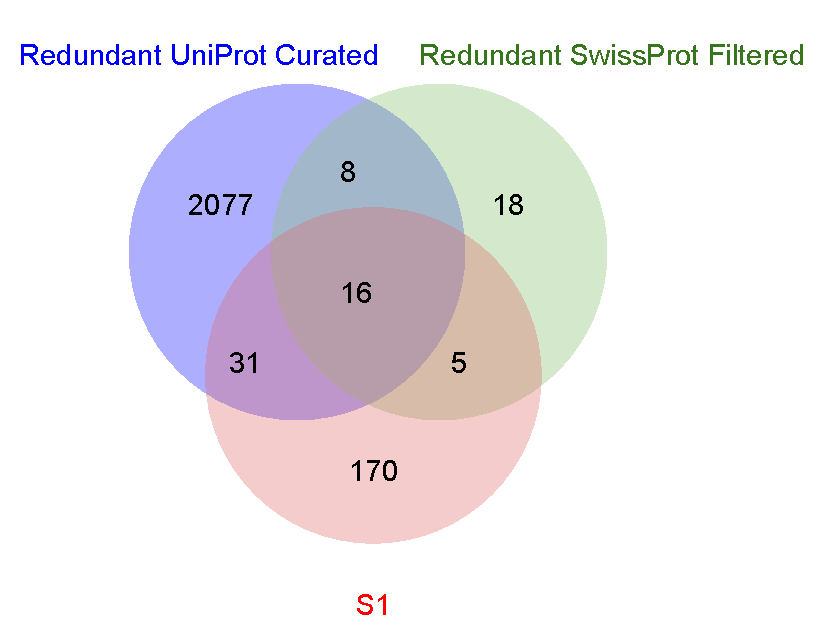
\includegraphics[width=1\textwidth]{TA_chapter/database-overlap}
        \captionof{figure}[A Venn diagram showing tail-anchored protein UniProt ids present in each of the datasets as well as those present in multiple datasets.]{\textbf{A Venn diagram showing tail-anchored protein UniProt ids present in each of the datasets as well as those present in multiple datasets.}
The number of ids present in redundant versions of
i) the supplementary materials table of a previous study predicting the complete set of human tail-anchored proteins denote by S1~\cite{Kalbfleisch2007} in red,
ii) and in green is the SwissProt dataset filtered according to typical~\gls{ta} features limited to the human proteome~\cite{TheUniProtConsortium2014}, and
iii) in blue is the UniProt curated list of~\gls{ta} proteins~\cite{TheUniProtConsortium2014}.
Note that to avoid losing IDs to redundancy reduction this diagram was generated without the use of CD-HIT~\cite{Huang2010, Wu2011}, which is applied in the later statistical analysis.}

\label{fig:tadatasetoverlap}
\end{figure}

In order to get an understanding of the consistency of the datasets, before removing redundant proteins, we compared these two datasets to a dataset remapped set of proteins from a previous 2007 method~\cite{Kalbfleisch2007}.
The S1 dataset was built with an aim to gather \gls{ta} proteins in the human genome from the NCBI.
The greatest source of uncertainty here is that the original S1 list includes 411 records, however, only 222 of these were successfully mapped to the UniProt dataset.
This figure is closer to the 202 proteins from the original S1 list that excluded proteins that were either hypothetical or splice isoforms.
That being said, this mapping step prevents us from directly comparing the entire original S1 dataset.
We compared the up-to-date datasets to S1 to see how many records are shared, how many are now obsolete, and how many are unique.

Figure~\ref{fig:tadatasetoverlap} shows that S1 has 175 record ids of 222 records (78.8\%) which do not share overlap the up-to-date manually curated UniProt dataset~\cite{TheUniProtConsortium2014}.
Of the 170 unique records of that S1 dataset, 4 were manually annotated as not belonging to the human proteome, 20 have the C terminal as annotated being cytoplasmic, only 125 had \texttt{TRANSMEM} annotation indicating a bona fide \gls{tmh}.
If we apply equivalent filters, only 42 have annotation verifying that they are \gls{ta} proteins.

Equivalent criteria to the original Kalbfleisch \textit{et al.,} 2007 \cite{Kalbfleisch2007} study were applied to the entire SwissProt database and then restricted to the human proteome dataset.
24 of these 47 records (51.1\%) are in the curated UniProt~\gls{ta}  dataset.
21 of the 49 (44.7\%) records from SwissProt filtered human dataset can be found in the original S1 list.

The same method applied to an up-to-date dataset overlaps more with a manually curated dataset.
There is also a large degree of what we now believe to be mistakes that occurred in the older prediction tools and datasets, even when using similar methods.
As a trend, this shows that up-to-date datasets improve the reliability of this automated predicted method.
These automated criteria still do not fully align with the manually curated list.
Of 2633 records, only 2241 have the \texttt{TRANSMEM} annotation.
Ultimately, this points to the idea that datasets are a moving target as they are constantly updated with more accurate information using evermore reliable tools and methods.

\subsection{It Is Difficult To Observe Any Hydrophobic Variation Of TA Protein TMHs From Different Species}

In single\--pass proteins of eukaryotic species, there are typically various adaptations of the \gls{tmh} to adhere to the membrane constraints of the specific membrane.
For single\--pass proteins, previous studies have observed differences in terms of \gls{tmh} hydrophobicity between yeast and human \gls{tmp}s~\cite{Sharpe2010}, or in cress, yeast, bacteria, and human datasets~\cite{Baker2017}.
We would expect to see a similar trend between the \gls{tmh}s of \gls{ta} proteins from different species.
However, when assuming a zero-difference hypothesis, in these \gls{tmh} \gls{ta} protein datasets we cannot observe any species-level differences between the datasets at this sample size for \gls{tmh} hydrophobicity.

When comparing the average Kyte \& Doolittle~\cite{Kyte1982} hydrophobicity values for the~\gls{tmh}s from humans and mice, \textit{A. thaliana}, and  \textit{S. cerevisiae}, we can see little difference between the mean values.
All of the mean values lie between 2.3-2.6 when we only consider the \gls{tmh} and at 1.3-1.6 when considering residues in close proximity to the~\gls{tmh} ($\pm$5 residues) (Figure~\ref{fig:average_species_hydrophobicity_ta}).

\begin{figure}[!ht]
\centering
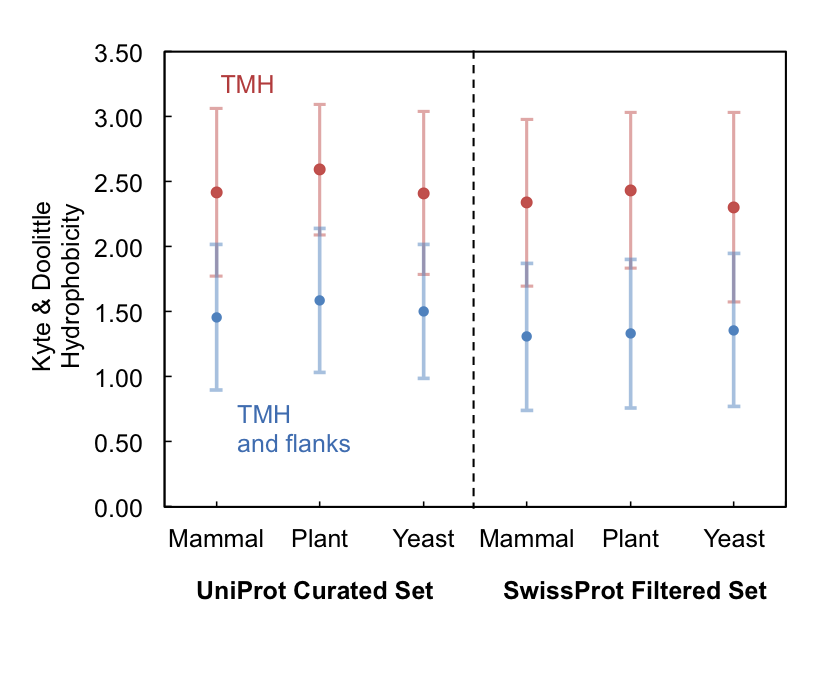
\includegraphics[width=1\textwidth]{TA_chapter/species-hydrophobicity}
\captionof{figure}[Average values of species datasets from UniProt manually curated set and SwissProt automatically filtered dataset.]
{\textbf{Average values of species datasets from UniProt manually curated set and SwissProt automatically filtered dataset.}

The average hydrophobicity values from the Kyte \& Doolittle scale~\cite{Kyte1982}.for both the \gls{tmh} and the \gls{tmh}$\pm$5 residues.
Values are shown for both the UniProt manually curated set and the SwissProt filtered set. In the UniProt manually curated set we compare the mammalian set of \gls{ta} proteins (Human N=30 and Mouse N=30) to \textit{A. thaliana} (N=57) representing plants and \textit{S. cerevisiae} (N=27) representing yeasts. For the SwissProt filtered set we compare the mammalian set of \gls{ta} proteins (Human N=46 and Mouse N=48) to \textit{A. thaliana} (N=49) representing plants  and  \textit{S. cerevisiae} (N=24) representing yeasts.
Error bars are shown at $\pm 1 \sigma$ from the mean of the respective dataset.
}

\label{fig:average_species_hydrophobicity_ta}
\end{figure}

Indeed, we see no strong observable statistical differences in hydrophobicity ($P>3.35E-1$ in the SwissProt automatically filtered list Table \ref{table:speciestableswissprotstats}, and $P>2.40E-1$ in the UniProt curated list Table \ref{table:speciestableuniprotstats}).
There are also no consistent trends among the absolute Bahadur slopes; no datasets are greatly different from any other.

\begin{table}[htbp]
\centering
\captionof{table}[Hydrophobicity statistical comparisons between mouse and human, yeast, and plants in the SwissProt Filtered Dataset.]
{\textbf{Hydrophobicity statistical comparisons between mouse and human, yeast, and plants in the SwissProt Filtered Dataset.}
Here, we compare a mammalian set of \gls{ta} proteins (Human N=46 and Mouse N=48) to \textit{A. thaliana} (N=49) representing plants  and  \textit{S. cerevisiae} (N=24) representing yeasts.
The hydrophobicity was predicted as the mean average of the values of the sequences of the \gls{tmh}, as well another group including up to $\pm$5 flanking residues, since predicting the boundary of \gls{tmh}s is difficult, according to the Kyte \& Doolittle hydrophobicity scale~\cite{Kyte1982}.
The Test column refers to the statistical score obtained from the test; H statistic for the Kruskal Wallis, the KS statistic for the Kolmogorov Smirnov test, and the t-statistic for the T-test.
$P$ is the P-value of that statistical score.
$B$ refers to the Bahadur slope, an interpretation of the P-value that accounts for the sample size powering the test~\cite{Bahadur1967, Bahadur1971}.}
\tiny
    % Table generated by Excel2LaTeX from sheet 'SwissProt filtered species'

    \begin{tabular}{clrrrrrrrrr}
          &       & \multicolumn{3}{c}{Mammal and Plant} & \multicolumn{3}{c}{Mammal and Yeast} & \multicolumn{3}{c}{Plant and Yeast} \\
          &       & \multicolumn{1}{l}{Test} & \multicolumn{1}{l}{$P$} & \multicolumn{1}{l}{$B$} & \multicolumn{1}{l}{Test} & \multicolumn{1}{l}{$P$} & \multicolumn{1}{l}{$B$} & \multicolumn{1}{l}{Test} & \multicolumn{1}{l}{$P$} & \multicolumn{1}{l}{$B$} \\
    \multirow{3}[0]{*}{TMH } &  KW & 0.93  & 3.35E-1 & 7.64E-3 & 0.10  & 7.56E-1 & 2.37E-3 & 0.84  & 3.60E-1 & 1.40E-2 \\
          &  KS & 0.13  & 6.36E-1 & 3.17E-3 & 0.12  & 9.24E-1 & 6.69E-4 & 0.19  & 5.28E-1 & 8.76E-3 \\
          &  T-test & -0.86 & 3.90E-1 & 6.58E-3 & 0.21  & 8.31E-1 & 1.57E-3 & 0.79  & 4.33E-1 & 1.15E-2 \\
    \multirow{3}[0]{*}{TMH and flanks } &  KW & 0.04  & 8.52E-1 & 1.12E-3 & 0.12  & 7.28E-1 & 2.69E-3 & 0.04  & 8.33E-1 & 2.51E-3 \\
          &  KS & 0.11  & 7.72E-1 & 1.81E-3 & 0.13  & 8.79E-1 & 1.09E-3 & 0.11  & 9.80E-1 & 2.81E-4 \\
          &  T-test & -0.22 & 8.23E-1 & 1.37E-3 & -0.38 & 7.04E-1 & 2.97E-3 & -0.19 & 8.50E-1 & 2.22E-3 \\
    \end{tabular}%
                \label{table:speciestableswissprotstats}

\end{table}%

\begin{table}[htbp]
\centering
\captionof{table}[Hydrophobicity statistical comparisons between mouse and human, yeast, and plants in the UniProt Curated Dataset.]
{\textbf{Hydrophobicity statistical comparisons between mouse and human, yeast, and plants in the UniProt Curated Dataset.}
Here, we compare a mammalian set of \gls{ta} proteins (Human N=30 and Mouse N=30) to \textit{A. thaliana} (N=53) representing plants  and  \textit{S. cerevisiae} (N=27) representing yeasts.
The hydrophobicity was predicted as the mean average of the values of the sequences of the \gls{tmh}, as well another group including up to $\pm$5 flanking residues, since predicting the boundary of \gls{tmh}s is difficult, according to the Kyte \& Doolittle hydrophobicity scale~\cite{Kyte1982}.
The Test column refers to the statistical score obtained from the test; H statistic for the Kruskal Wallis, the KS statistic for the Kolmogorov Smirnov test, and the t-statistic for the T-test.
$P$ is the P-value of that statistical score.
$B$ refers to the Bahadur slope, an interpretation of the P-value that accounts for the sample size powering the test~\cite{Bahadur1967, Bahadur1971}.}
    \tiny
    % Table generated by Excel2LaTeX from sheet 'SwissProt filtered species'

    \begin{tabular}{clrrrrrrrrr}
                &       & \multicolumn{3}{c}{Mammal and Plant} & \multicolumn{3}{c}{Mammal and Yeast} & \multicolumn{3}{c}{Plant and Yeast} \\
                &       & \multicolumn{1}{l}{Test} & \multicolumn{1}{l}{P} & \multicolumn{1}{l}{B} & \multicolumn{1}{l}{Test} & \multicolumn{1}{l}{P} & \multicolumn{1}{l}{B} & \multicolumn{1}{l}{Test} & \multicolumn{1}{l}{P} & \multicolumn{1}{l}{B} \\
    \multirow{3}[0]{*}{TMH} &  KW & 0.71  & 4.01E-01 & 8.09E-03 & 0.03  & 8.72E-01 & 1.57E-03 & 0.57  & 4.48E-01 & 1.00E-02 \\
                &  KS & 0.13  & 6.93E-01 & 3.24E-03 & 0.13  & 9.11E-01 & 1.08E-03 & 0.20  & 4.16E-01 & 1.10E-02 \\
                &  T-test & -0.93 & 3.55E-01 & 9.15E-03 & -0.11 & 9.13E-01 & 1.04E-03 & 0.64  & 5.22E-01 & 8.12E-03 \\
    \multirow{3}[0]{*}{TMH and flanks} &  KW & 1.37  & 2.42E-01 & 1.26E-02 & 0.38  & 5.36E-01 & 7.17E-03 & 0.08  & 7.80E-01 & 3.11E-03 \\
                &  KS & 0.19  & 2.40E-01 & 1.26E-02 & 0.14  & 8.13E-01 & 2.38E-03 & 0.09  & 9.97E-01 & 3.21E-05 \\
                &  T-test & -1.17 & 2.45E-01 & 1.24E-02 & -0.79 & 4.35E-01 & 9.58E-03 & 0.20  & 8.43E-01 & 2.14E-03 \\
    \end{tabular}%
                    \label{table:speciestableuniprotstats}
    \end{table}%

Here, we are dealing with datasets at least an order of magnitude smaller than those broad studies \cite{Sharpe2010, Baker2017} which could explain the absence of the effect.
However, this only goes to show that if there is a biochemically distinct effect in \gls{ta} proteins in terms of hydrophobicity between species, it is indeed weak.


\subsection{There Are Biochemical Differences Between Tail-Anchored TMHs From Different Organelles}

As is typical in the case of species, \gls{tmh}s with different subcellular localisations on average have different hydrophobicity.
This could be in part due to the variation in membrane potential across the different organelles~\cite{Qin2011, Worley1994, Schapiro2000}, the known lipid asymmetry caused by sphingomyelin and glycosphingolipids on the non-cytosolic leaflet and phosphatidylserine and phosphatidylethanolamine in the cytosolic leaflet in the Golgi and \gls{pm} and lack of asymmetry in the \gls{er}~\cite{Daleke2007, Devaux2004}, or that sphingomyelin is not present in the \gls{er} but is present in the Golgi~\cite{Futerman2005} and \gls{pm}~\cite{Li2007, Tafesse2007}.
Furthermore, the \gls{pm} contains densely packed sphingolipids and sterols~\cite{Paolo2006}.
%Need a sentence on the mitochondrial membrane

%Need mitochondria reference, and numbers for the UniER etc.
These hydrophobic differences have already been observed in the mitochondria localised \gls{ta} protein \gls{tmh} \cite{Borgese2003}.
Here we consider the \gls{ta} proteins at certain locations within the cell ignoring species, and we see clear differences in the biochemistry of the \gls{tmh}.
In the UniProt manually curated dataset, the Kyte \& Doolittle hydrophobicity scores rage from 1.7 in mitochondria to 2.7 in the \gls{pm} (Figure \ref{fig:average_organelle_factors_ta}A).

\begin{figure}
\centering
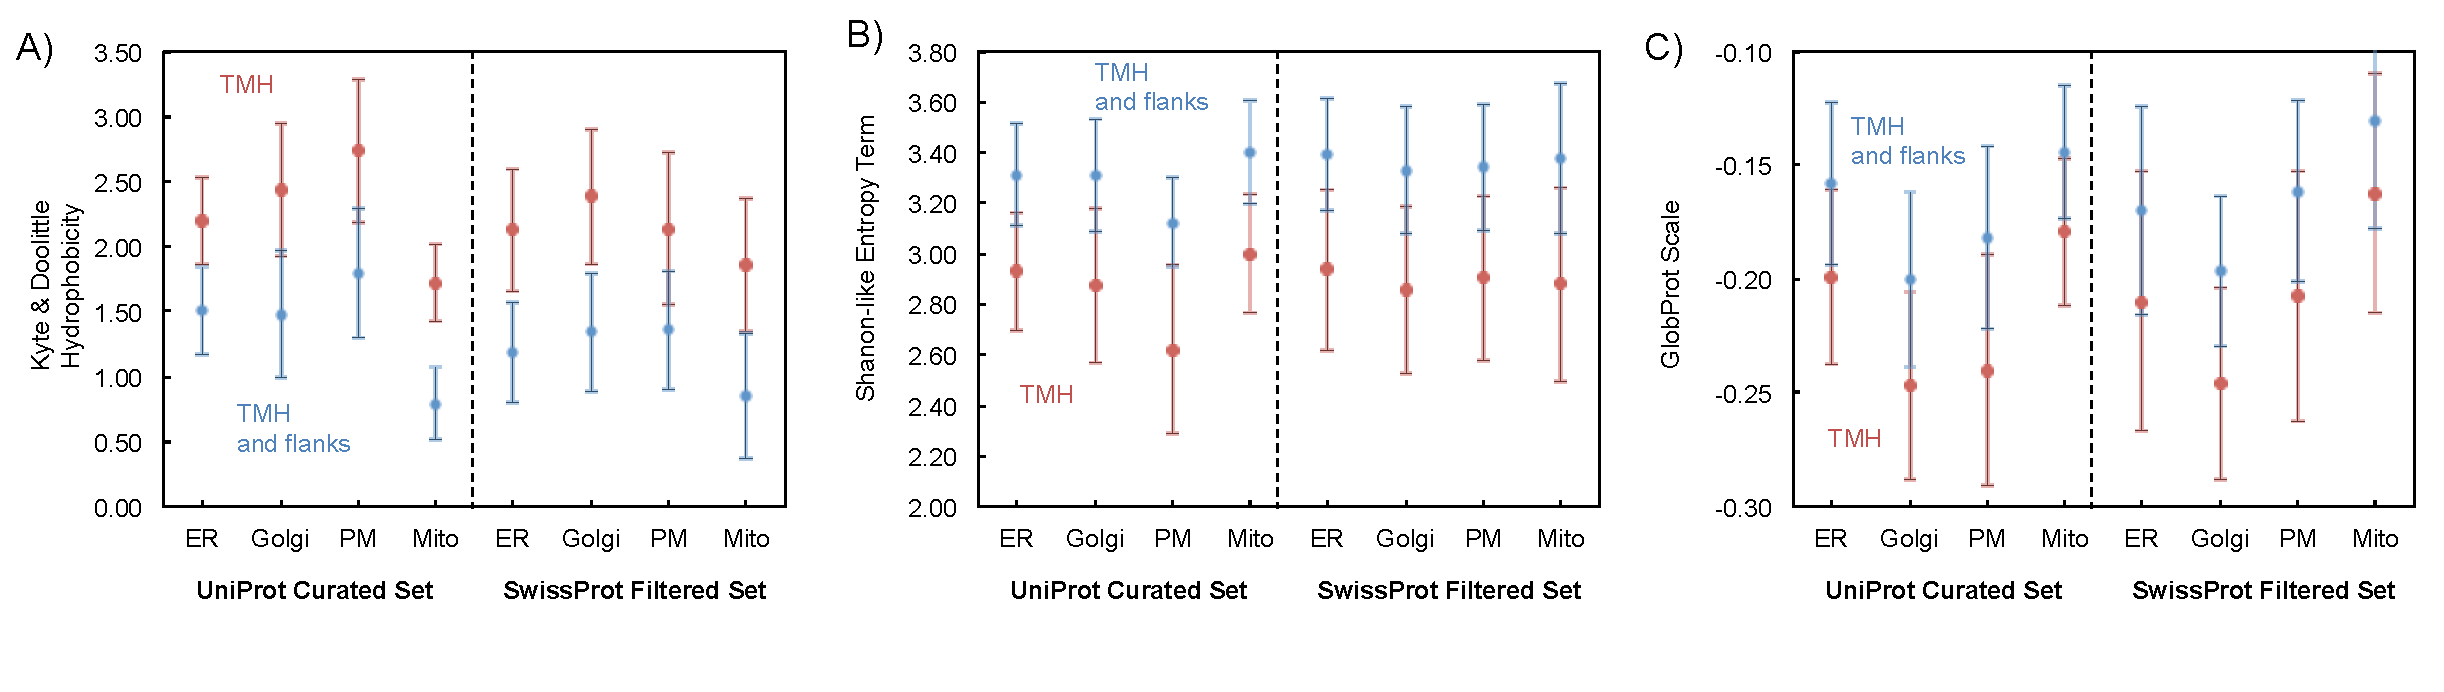
\includegraphics[width=0.75\textwidth]{TA_chapter/organelle-averages}
\captionof{figure}[Average sequence\--based biochemical values of organelle datasets from UniProt manually curated set and SwissProt automatically filtered dataset.]
{\textbf{Average sequence\--based biochemical values of organelle datasets from UniProt manually curated set and SwissProt automatically filtered dataset.}

A) The average hydrophobicity values from the Kyte \& Doolittle scale~\cite{Kyte1982}, B) the average information entropy~\cite{Shannon1948} (see methods) for both the \gls{tmh} and the \gls{tmh}$\pm$5 residues.
Values are shown for both the UniProt manually curated set and the SwissProt filtered set.
In the UniProt manually curated set we compare \gls{ta} proteins from the~\gls{er} (N=400) to the Golgi (N=82), the~\gls{pm} (N=37), and the mitochondria (N=401).
For the SwissProt filtered set we compare \gls{ta} proteins from the~\gls{er} (N=98) to the Golgi (N=82), the~\gls{pm} (N=157), and the mitochondria (N=65).
Error bars are shown at $\pm 1 \sigma$ from the mean of the respective dataset.
}

\label{fig:average_organelle_factors_ta}
\end{figure}







\begin{table}[htbp]
\centering
\captionof{table}[Statistical comparisons between TMH sequences from organelles in the UniProt Curated Dataset.]
{\textbf{Statistical comparisons between TMH sequences from organelles in the UniProt Curated Dataset.}
Here, we compare an organelle subset from the UniProt curated dataset of \gls{ta} proteins.
We compare \gls{er} (N=397) to Golgi (N=83), \gls{pm} (N=31), and the mitochondria (N=426).
The hydrophobicity was predicted as the mean average of the values of the sequences of the \gls{tmh}, as well another group including up to $\pm$5 flanking residues, since predicting the boundary of \gls{tmh}s is difficult, according to the Kyte \& Doolittle hydrophobicity scale~\cite{Kyte1982}.
The linguistic information entropy was calculated according to the methods section~\cite{Shannon1948}.
The Test column refers to the statistical score obtained from the test; H statistic for the Kruskal Wallis (KW), the KS statistic for the Kolmogorov Smirnov test (KS), and the t-statistic for the student's T-test (T-test).
$P$ is the P-value of that statistical score.
$B$ refers to the Bahadur slope, an interpretation of the P-value that accounts for the sample size powering the test~\cite{Bahadur1967, Bahadur1971}.}
    \tiny

    \begin{tabular}{clrrrrrrrrr}
                &       & \multicolumn{3}{c}{ER and Golgi} & \multicolumn{3}{c}{ER and PM} & \multicolumn{3}{c}{ER and mito} \\
                &       & \multicolumn{1}{l}{Test} & \multicolumn{1}{l}{P} & \multicolumn{1}{l}{B} & \multicolumn{1}{l}{Test} & \multicolumn{1}{l}{P} & \multicolumn{1}{l}{B} & \multicolumn{1}{l}{Test} & \multicolumn{1}{l}{P} & \multicolumn{1}{l}{B} \\
    \multirow{3}[0]{*}{Hydrophobicity of TMH } &  KW & 21.83 & 2.98E-06 & 2.66E-02 & 28.53 & 9.21E-08 & 3.80E-02 & 377.02 & 5.54E-84 & 2.34E-01 \\
                &  KS & 0.34  & 1.61E-07 & 3.27E-02 & 0.57  & 5.32E-09 & 4.47E-02 & 0.67  & 4.22E-82 & 2.28E-01 \\
                &  T-test & -6.45 & 2.72E-10 & 4.61E-02 & -8.86 & 2.30E-17 & 8.99E-02 & 23.53 & 6.58E-94 & 2.61E-01 \\
    \multirow{3}[0]{*}{... and flanks} &  KW & 0.21  & 6.48E-01 & 9.07E-04 & 17.53 & 2.83E-05 & 2.46E-02 & 490.46 & 1.13E-108 & 3.03E-01 \\
                &  KS & 0.19  & 1.10E-02 & 9.44E-03 & 0.50  & 4.69E-07 & 3.42E-02 & 0.82  & 5.58E-123 & 3.43E-01 \\
                &  T-test & 0.32  & 7.48E-01 & 6.07E-04 & -4.85 & 1.75E-06 & 3.11E-02 & 34.60 & 2.19E-162 & 4.53E-01 \\
    \multirow{3}[0]{*}{Sequence Entropy of TMH } &  KW & 4.66  & 3.09E-02 & 7.28E-03 & 27.54 & 1.54E-07 & 3.68E-02 & 24.03 & 9.48E-07 & 1.69E-02 \\
                &  KS & 0.24  & 4.78E-04 & 1.60E-02 & 0.46  & 4.20E-06 & 2.91E-02 & 0.18  & 2.10E-06 & 1.59E-02 \\
                &  T-test & 3.22  & 1.37E-03 & 1.38E-02 & 6.42  & 3.71E-10 & 5.10E-02 & -4.55 & 6.28E-06 & 1.46E-02 \\
    \multirow{3}[0]{*}{... and flanks} &  KW & 0.52  & 4.70E-01 & 1.58E-03 & 19.50 & 1.01E-05 & 2.70E-02 & 40.11 & 2.40E-10 & 2.70E-02 \\
                &  KS & 0.13  & 2.06E-01 & 3.31E-03 & 0.41  & 7.97E-05 & 2.22E-02 & 0.23  & 5.53E-10 & 2.60E-02 \\
                &  T-test & 1.08  & 2.82E-01 & 2.65E-03 & 4.47  & 1.00E-05 & 2.70E-02 & -5.84 & 7.51E-09 & 2.28E-02 \\
    \end{tabular}%
                    \label{table:organellesuniprotstats}
    \end{table}%

In the UniProt curated list, there are clear hydrophobic differences between all the organelle \gls{tmh} datasets excluding flanks ($P<2.98E-6$) which as a trend becomes less clear when considering the \gls{tmh}$\pm$5 flanking residues except for mitochondria which increases in significance when considering the flanks also (Table~\ref{table:organellesuniprotstats}).
The \gls{er} and mitochondrial tests are very significant ($P<4.22E-82$).
Consistently the Bahadur slope is at least an order of magnitude greater in the \gls{er} and mitochondrial comparison than for the other considerations, so these differences cannot be accounted for by the larger sample size.
This gap in hydrophobicity appears to be due to a trend of the \gls{er}, \gls{pm}, and Golgi using isoleucine, valine, and leucine as their most common \gls{tmh} residues, whereas in the case mitochondrial located \gls{ta} proteins, the most common residue type is alanine in the UniProt manually curated dataset (16.3\% of total residues) followed by valine (12\% total residues)(Figure \ref{fig:uniprot-heatmap}).

\begin{figure}
\centering
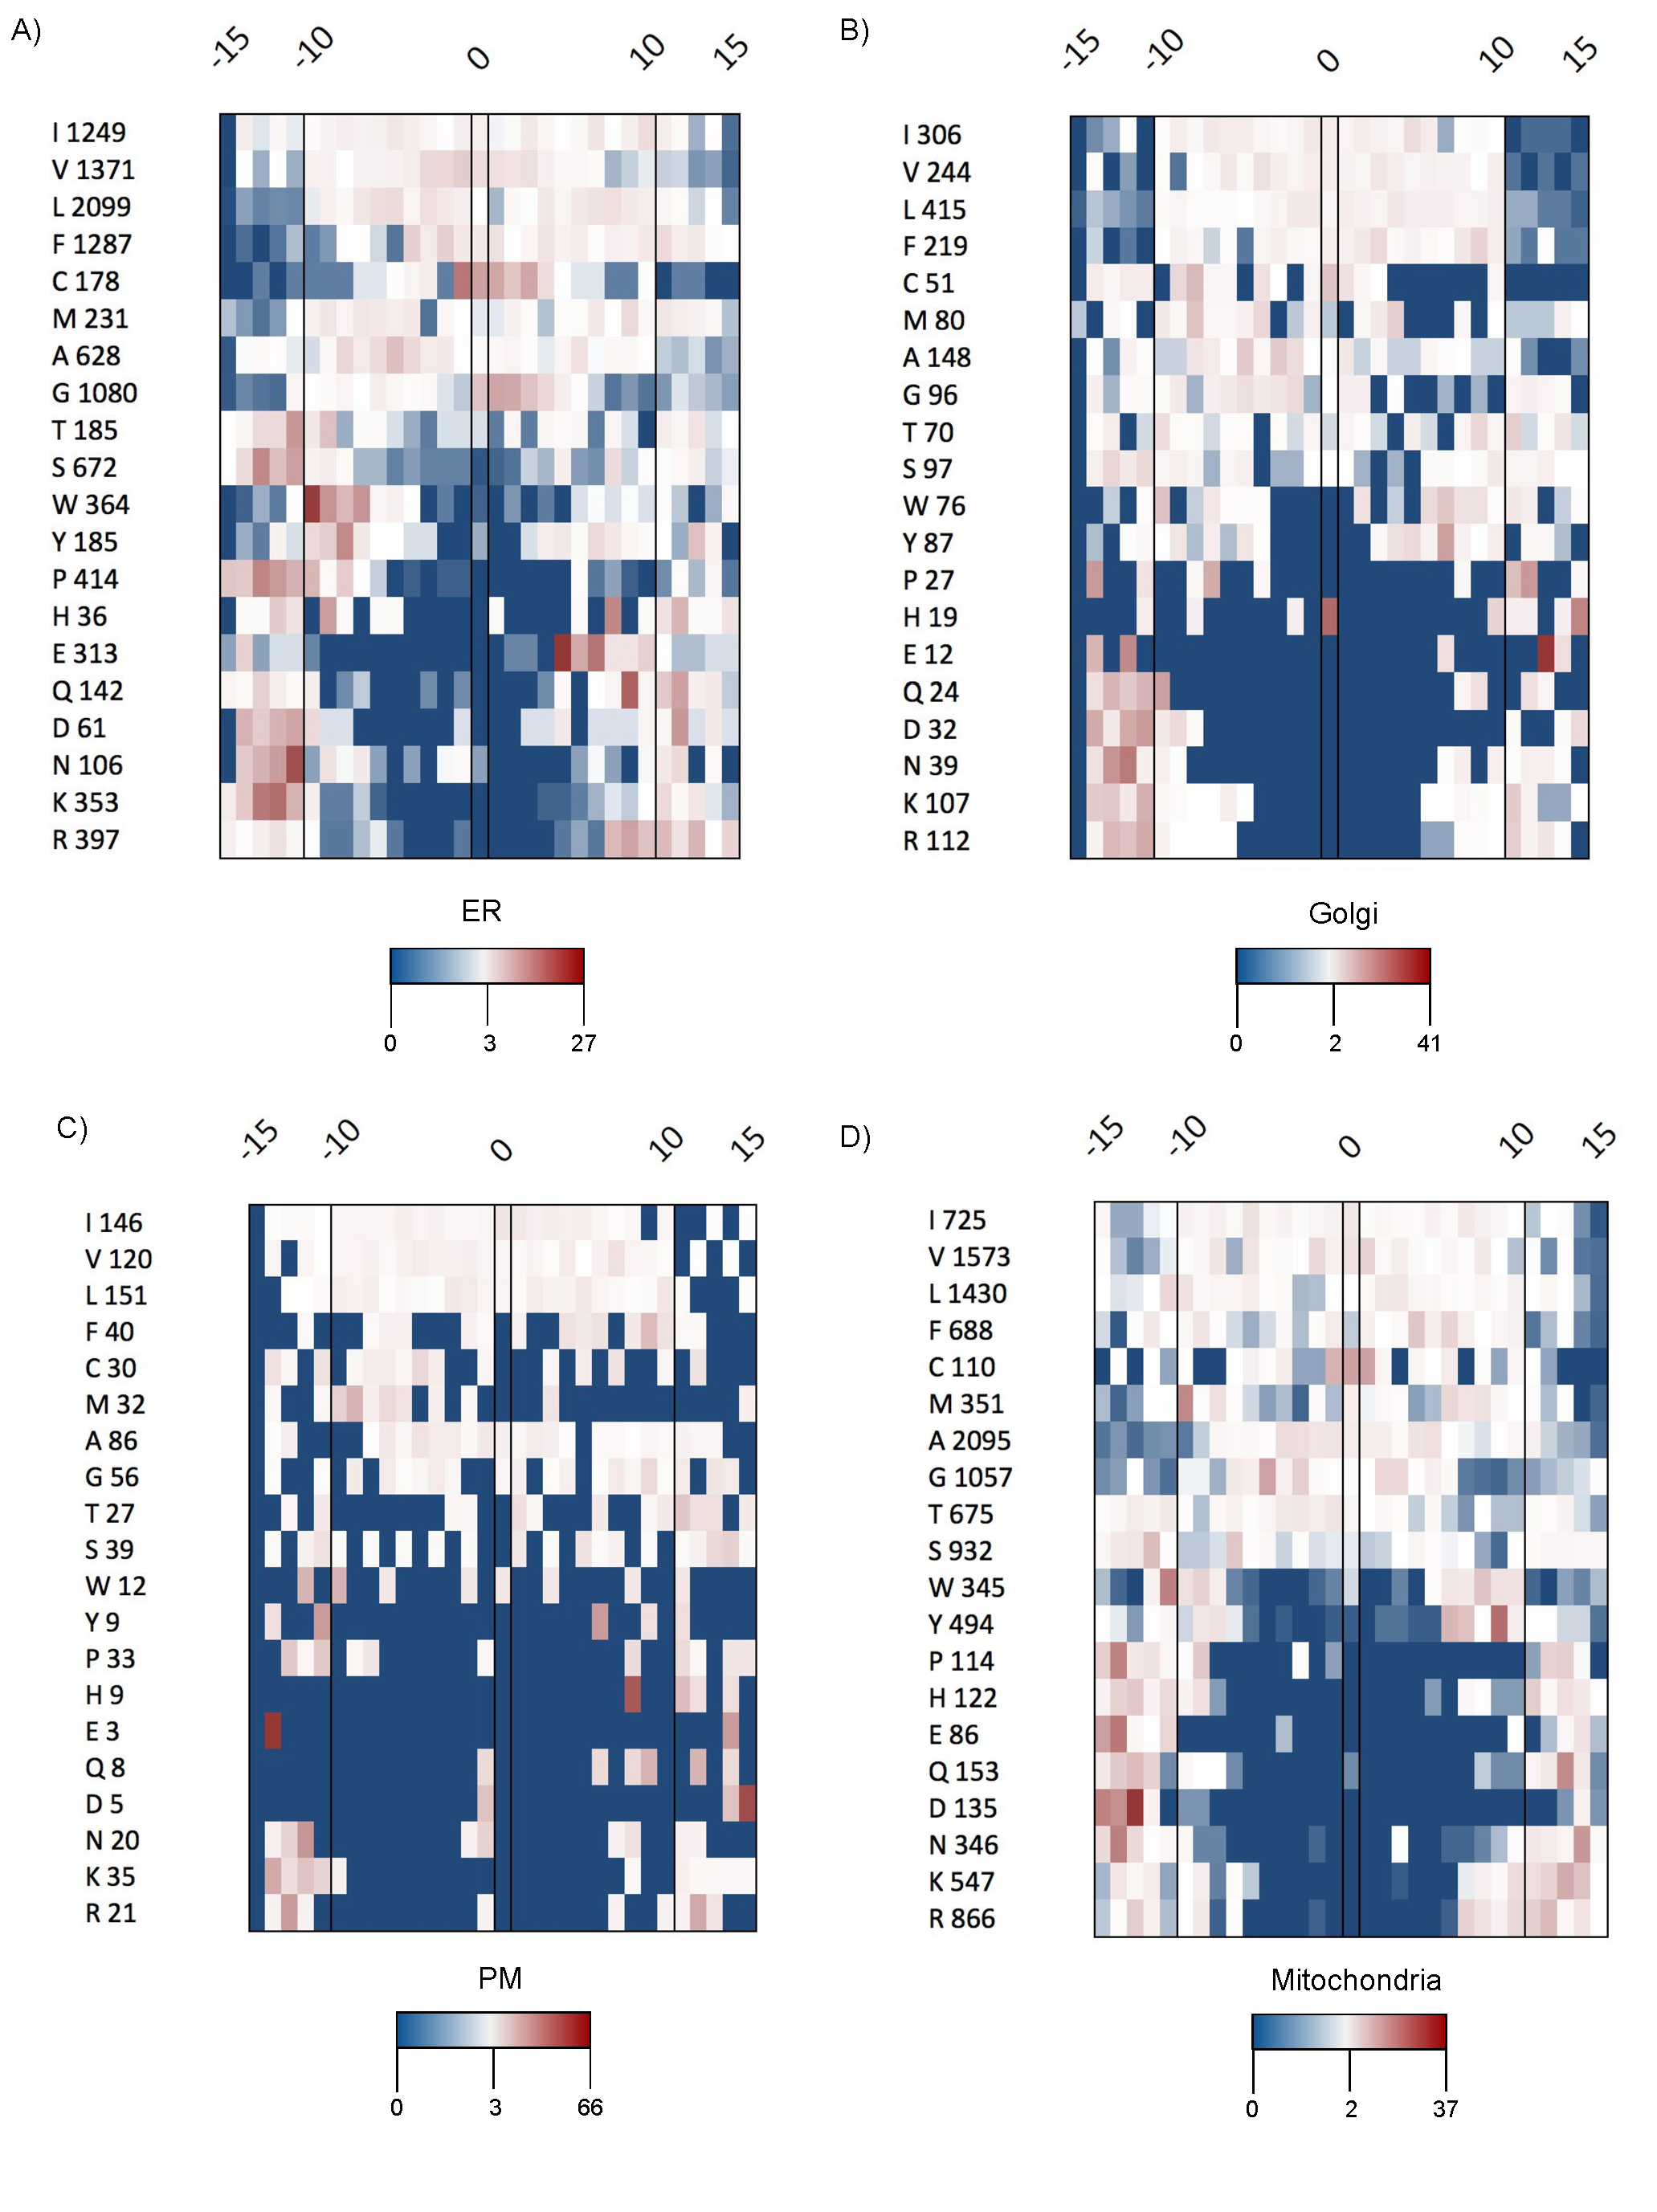
\includegraphics[width=1\textwidth]{TA_chapter/UniProt-heatmaps}
\captionof{figure}[The normalised skews of each amino acids from TA proteins grouped by localisation from the SwissProt automatically filtered dataset.]
{\textbf{The normalised skews of each amino acids from TA proteins grouped by localisation from the UniProt manually curated dataset.}

The residue position aligned with the centre of the TMH is on the horizontal axis, and the residue type is on the vertical axis.
Amino acid types are listed in order of decreasing hydrophobicity according to the Kyte and Doolittle scale \cite{Kyte1982}.
Flank lengths were restricted to $\pm$5 residues.
The edge residues from proteins with flank lengths and \gls{tmh} lengths that exceeded the plotted 31 residues were still included in the normalisation calculations despite not being plotted.
The colour scale represents the relative percentage of a particular amino acid and is shown with dark blue as 0, white as the 50th percentile value of the entire heatmap, and dark red as the highest percentage on the heat map.
The panels are constructed from TA proteins derived from the SwissProt automatic method with redundancy removal applied detailed in the methods section.
The datasets were further separated by subcellular locations: (a) the \gls{er}, (b) the Golgi, (c) the cell membrane, (d) the mitochondria.
These datasets are more thoroughly outlined in the methods section.
}

\label{fig:uniprot-heatmap}
\end{figure}

Similarly, alanine is the second most common residue in mitochondrial located \gls{ta} proteins from the Swissprot automatically generated dataset at 11.9\% of the total residues after leucine which is 13.4\% of the total residues(Figure \ref{fig:swissprot-heatmap}).

Analysis from 16 \gls{ta} proteins with known subcellular locations showed that both the C-terminal tail charge and hydrophobicity are determinates of the terminal destination to the \gls{er}, mitochondria, and the peroxisome intra-cellular sub-cellular locations \cite{Costello2017}.
They found that less hydrophobicity and more charge in the ``tail'' determined the \gls{ta} protein for the mitochondria rather than the \gls{er}.
This corroborates what we see in terms of hydrophobicity (Figure \ref{fig:average_organelle_factors_ta}A).
When we consider charge difference between organelles on larger datasets, we see trends that reinforce this idea, however, rather than net charge, we see charge distribution along the \gls{tmh} and the neighbouring flanks.
In the Swissprot automatically filtered dataset, in the \gls{er} 9.4\% of the residues are positively charged, and 2.5\% are negatively charged.
Most of the positively charged residues cluster following the ``positive\--inside'' rule between positions -15 and -10 for R and K, but so do the negatively charged residues D and E, effectively reducing this local charge by 2.5\%.
In mitochondria, we find that the proportion of charge is similar (10.4\% R and K, 3.3\% D and E) however the negatively charged residues cluster on the N flank (-15 to -8) and the positively charged residues cluster more strongly on the outside flank (positions 9 to 15) (Figure \ref{fig:swissprot-heatmap}).

In the UniProt manually curated \gls{er} set, 6.6\% of residues are positively charged and 3.3\% of residues are negatively charged.
K clusters strongly on the inside flank as expected, yet R clusters strongly between positions 7 to 15 and rather weakly at the inside flank (positions -15 to -10) (Figure \ref{fig:uniprot-heatmap}).
Similarly to the SwissProt sets, D prefers the inside flank but is tolerated in the outside flank.
The more abundant E residues behave very unusually and cluster at positions 5-10.
Generally, charged residues are suppressed in the \gls{tmh} core \cite{Sharpe2010, Baeza-Delgado2013}, especially in anchoring \gls{tmh}s \cite{Baker2017}.
It is unclear why this is observed, yet, altogether the 313 glutamic acid residues and 397 arginine residues that appear unusually deep in the \gls{tmh} core may be to an extent neutralising one another in the folded \gls{tmh} arrangement, but are ultimately not that abundant compared to the total number of residues in this organelle dataset (11351 total residues).
In mitochondria, 1413 positively charged residues (11\% of the total residues in the mitochondrial dataset) were preferentially located at the outside flank and somewhat into the core (positions 6 to 15) than the expected ``inside'' flank (positions -15 to -5).
The 221 negatively charged residues (1.7\%) unusually cluster at the inside.
This results in a strong net positive\--outside charge signal.

\begin{figure}
\centering
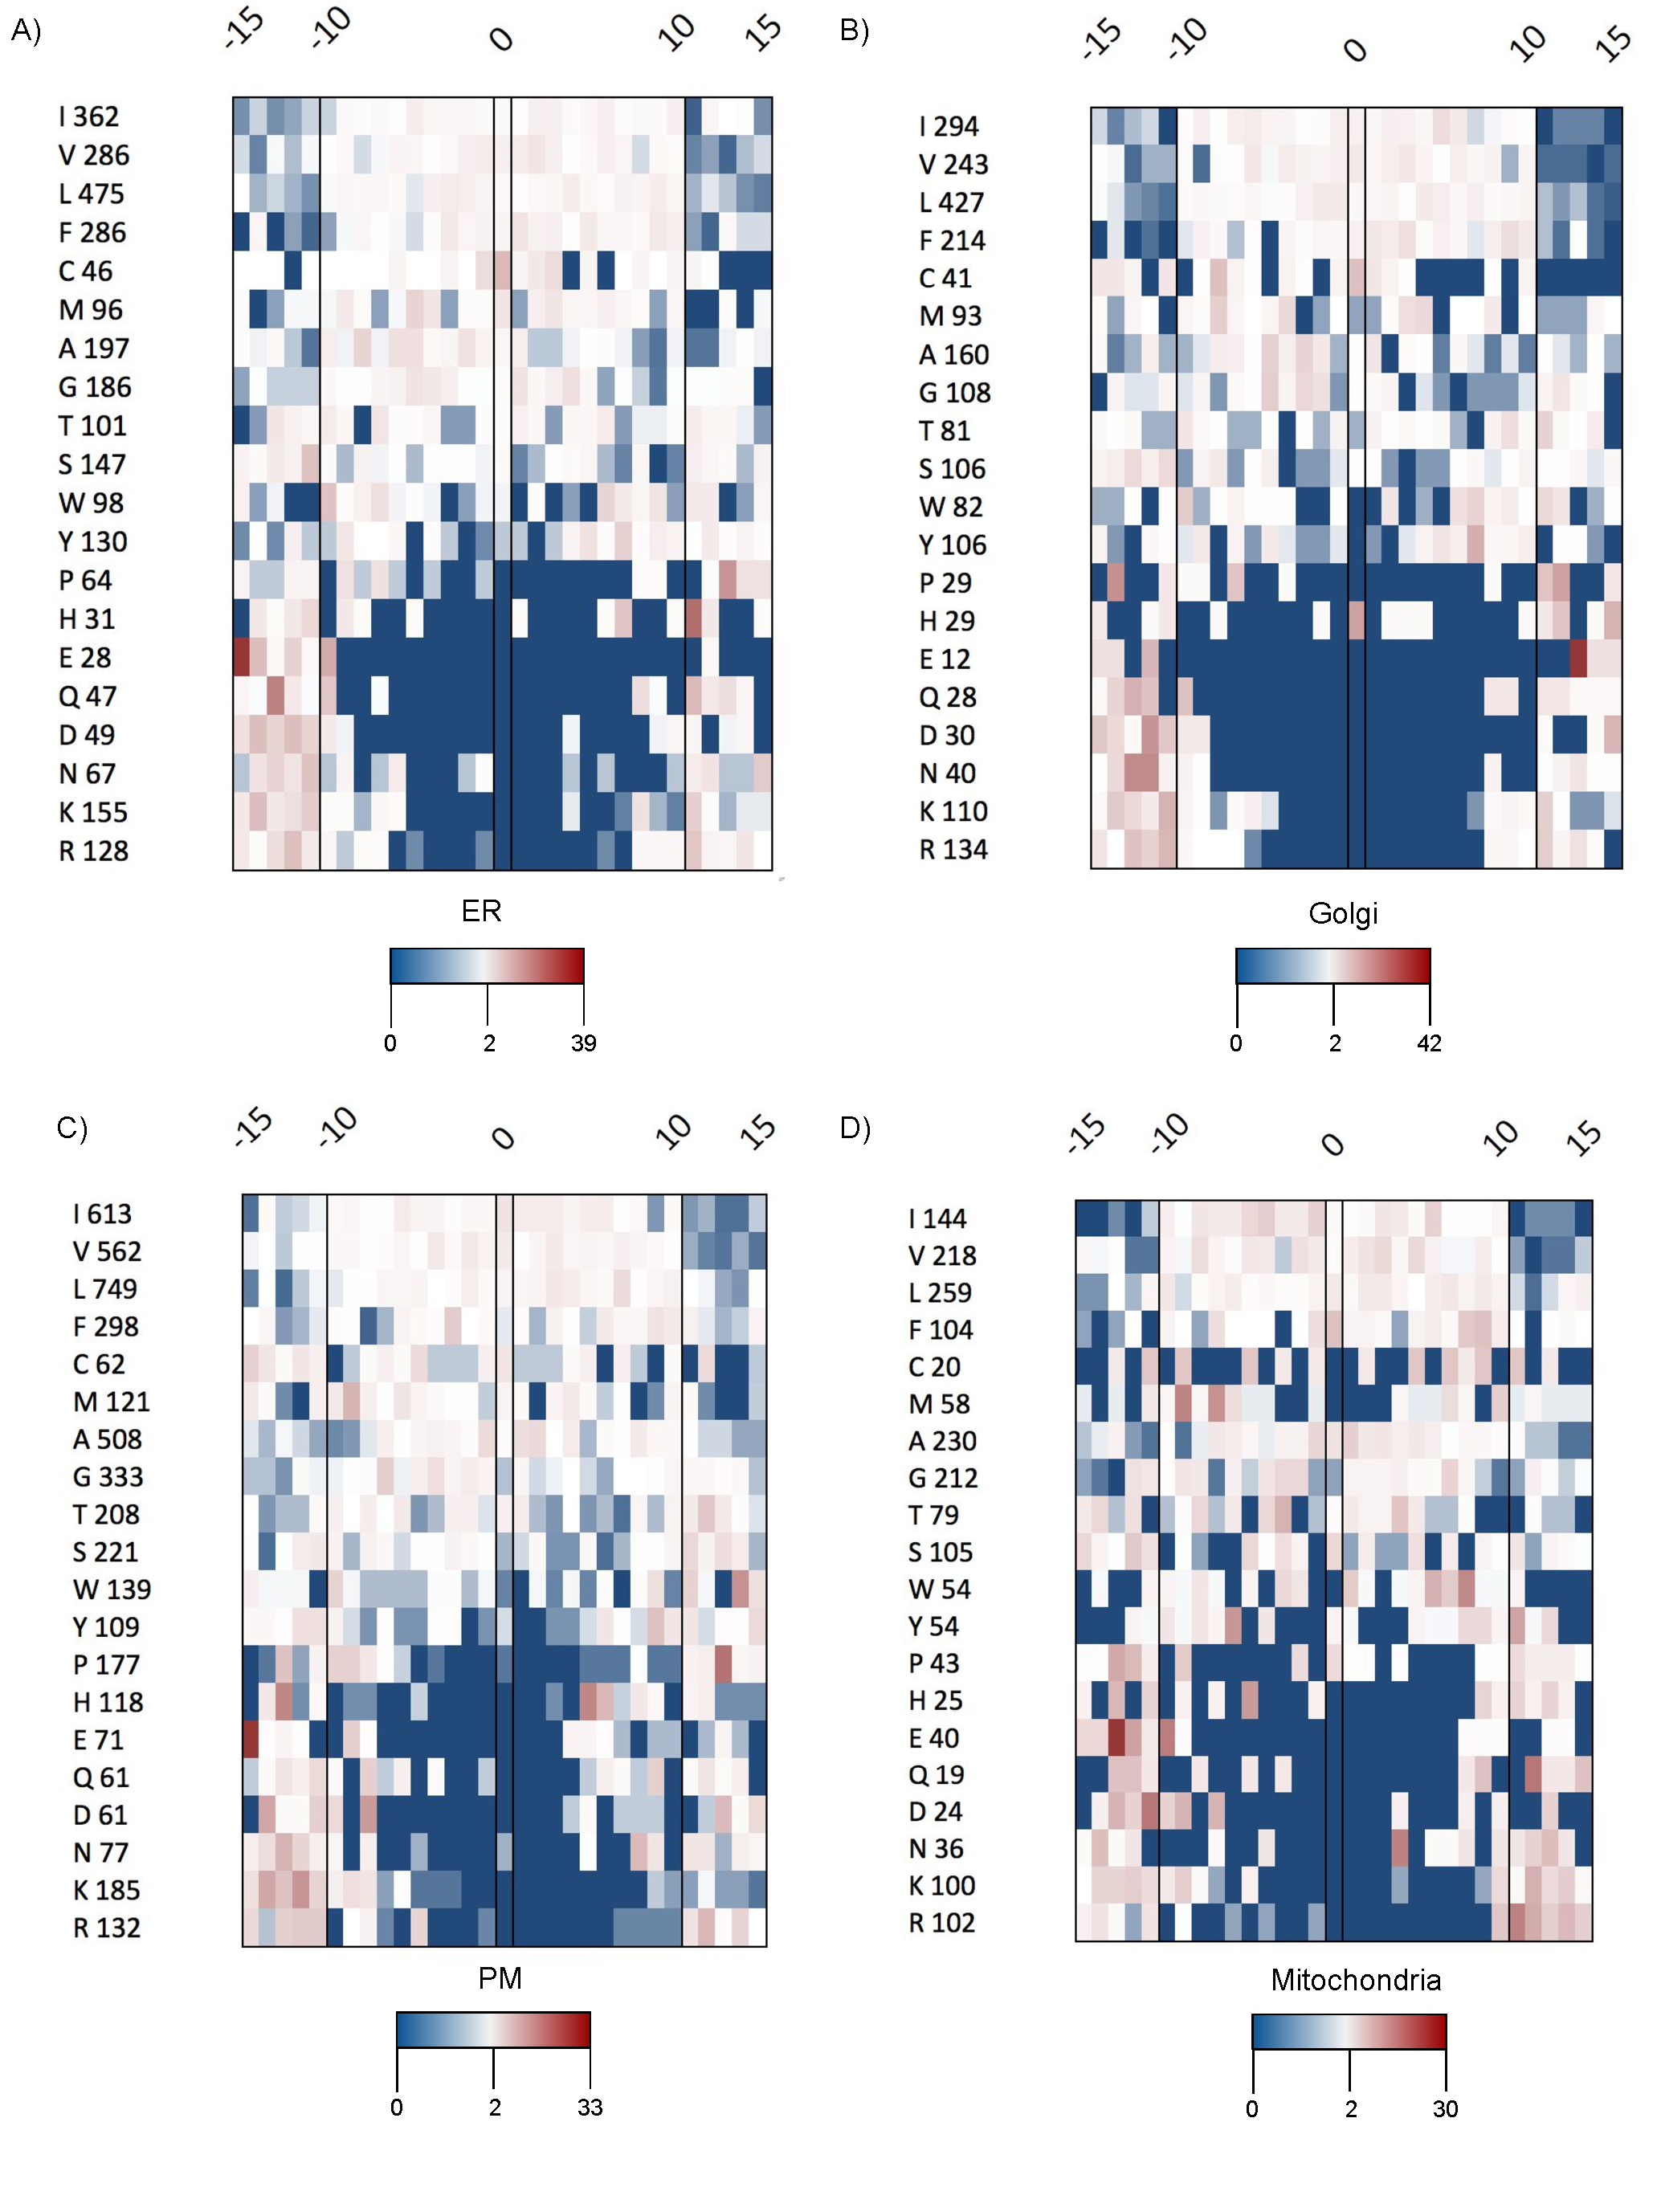
\includegraphics[width=1\textwidth]{TA_chapter/SwissProt-heatmaps}
\captionof{figure}[The normalised skews of each amino acids from TA proteins grouped by localisation from the SwissProt automatically filtered dataset.]
{\textbf{The normalised skews of each amino acids from TA proteins grouped by localisation from the SwissProt automatically filtered dataset}

Similarly to figure \ref{fig:uniprot-heatmap}, the residue position aligned with the centre of the TMH is on the horizontal axis, and the residue type is on the vertical axis.
Amino acid types are listed in order of decreasing hydrophobicity according to the Kyte and Doolittle scale \cite{Kyte1982}.
Flank lengths were restricted to $\pm$5 residues.
The edge residues from proteins with flank lengths and \gls{tmh} lengths that exceeded the plotted 31 residues were still included in the normalisation calculations despite not being plotted.
The colour scale represents the relative percentage of a particular amino acid and is shown with dark blue as 0, white as the 50th percentile value of the entire heatmap, and dark red as the highest percentage on the heat map.
The panels are constructed from TA proteins derived from the SwissProt automatic method with redundancy removal applied detailed in the methods section.
The datasets were further separated by subcellular locations: (a) the \gls{er}, (b) the Golgi, (c) the cell membrane, (d) the mitochondria.
These datasets are more thoroughly outlined in the methods section.
}

\label{fig:swissprot-heatmap}
\end{figure}

Information entropy has been known to identify cryptic function in \gls{tmh}s when considered along with hydrophobicity \cite{Wong2011, Wong2012}.
In terms of information entropy, there is a marked decrease in entropy in the \gls{pm} subset (mean entropy = 3.15 in the \gls{tmh}, 2.67 including $\pm$5 flanking residues) from the UniProt curated dataset compared to the other organelle datasets (entropy $>$ 3.29 and $>$ 2.85 including the flanks).
However, this stark difference between \gls{tmh}s from \gls{pm} bound \gls{ta} proteins and the other organelle datasets cannot be observed in the SwissProt set (Figure~\ref{fig:average_organelle_factors_ta}).

No clear significant differences can be observed for the information entropy ($P>6.33E-2$).
This is unsurprising given that the hydrophobic nature of the \gls{tmh}s demands that certain residues must be over-represented, which lowers the information entropy.
In this case, we have a highly hydrophobic set, the \gls{pm} UniProt set, which likely contains a higher proportion of the most hydrophobic residues.
As a trend, the information entropy mirrors the hydrophobicity albeit with less range between dataset means (2.67-3.15 in the \gls{tmh} for information entropy, 1.72-2.74 for hydrophobicity)(Figure~\ref{fig:average_organelle_factors_ta}).


    \begin{table}[htbp]
    \centering
    \captionof{table}[Statistical comparisons between TMH sequences from organelles in the SwissProt Filtered Dataset.]
    {\textbf{Statistical comparisons between TMH sequences from organelles in the SwissProt Filtered Dataset.}
    Here, we compare organelle subsets from the SwissProt automatically filtered dataset of \gls{ta} proteins.
    We compare \gls{er} (N=98) to Golgi (N=82), \gls{pm} (N=157), and the mitochondria referred to as ``mito'' (N=65).
    The hydrophobicity was predicted as the mean average of the values of the sequences of the \gls{tmh}, as well another group including up to $\pm$5 flanking residues, since predicting the boundary of \gls{tmh}s is difficult, according to the Kyte \& Doolittle hydrophobicity scale~\cite{Kyte1982}.
    The linguistic information entropy was calculated according to the methods section~\cite{Shannon1948}.
    The Test column refers to the statistical score obtained from the test; H statistic for the Kruskal Wallis (KW), the KS statistic for the Kolmogorov Smirnov test (KS), and the t-statistic for the student's T-test (T-test).
    $P$ is the P-value of that statistical score.
    $B$ refers to the Bahadur slope, an interpretation of the P-value that accounts for the sample size powering the test~\cite{Bahadur1967, Bahadur1971}.}
        \tiny
        % Table generated by Excel2LaTeX from sheet 'SwissProt filtered species'

        %\begin{tabular}{clrrrrrrrrr}
         \begin{tabular}{ccccccccccc}
                                &       & \multicolumn{3}{c}{ER and Golgi} & \multicolumn{3}{c}{ER and PM} & \multicolumn{1}{l}{ER and mito} &       &  \\
                                &       & \multicolumn{1}{l}{Test} & \multicolumn{1}{l}{$P$} & \multicolumn{1}{l}{$B$} & \multicolumn{1}{l}{Test} & \multicolumn{1}{l}{$P$} & \multicolumn{1}{l}{$B$} & \multicolumn{1}{l}{Test} & \multicolumn{1}{l}{$P$} & \multicolumn{1}{l}{$B$} \\

        \midrule
        \multirow{3}[0]{*}{TMH Hydrophobicity} &  KW & 11.96 & 5.43E-4 & 4.18E-2 & 0.02  & 8.77E-1 & 5.14E-4 & 8.46  & 3.64E-3 & 3.45E-2 \\
                                &  KS & 0.27  & 1.98E-3 & 3.46E-2 & 0.08  & 8.48E-1 & 6.44E-4 & 0.27  & 4.62E-3 & 3.30E-2 \\
                                &  T-test & -3.47 & 6.50E-4 & 4.08E-2 & -0.17 & 8.67E-1 & 5.60E-4 & 3.45  & 7.24E-4 & 4.44E-2 \\
        \midrule
        \multirow{3}[0]{*}{... including flanks} &  KW & 5.92  & 1.50E-2 & 2.33E-2 & 9.14  & 2.50E-3 & 2.35E-2 & 26.42 & 2.75E-7 & 9.27E-2 \\
                                &  KS & 0.21  & 2.85E-2 & 1.98E-2 & 0.26  & 4.88E-4 & 2.99E-2 & 0.43  & 4.93E-7 & 8.91E-2 \\
                                &  T-test & -2.52 & 1.25E-2 & 2.43E-2 & -3.09 & 2.23E-3 & 2.40E-2 & 4.95  & 1.87E-6 & 8.09E-2 \\
      \midrule

        \multirow{3}[0]{*}{TMH entropy} &  KW & 2.96  & 8.56E-2 & 1.37E-2 & 0.66  & 4.17E-1 & 3.43E-3 & 0.69  & 4.05E-1 & 5.54E-3 \\
                                &  KS & 0.13  & 4.32E-1 & 4.66E-3 & 0.10  & 5.27E-1 & 2.51E-3 & 0.18 & 1.40E-1 & 1.20E-2 \\
                                &  T-test & 1.58  & 1.15E-1 & 1.20E-2 & 0.79  & 4.32E-1 & 3.29E-3 & 1.03 & 3.06E-1 & 7.26E-3 \\
        \midrule
        \multirow{3}[0]{*}{... including flanks} &  KW & 2.62  & 1.06E-1 & 1.25E-2 & 2.87  & 9.04E-2 & 9.42E-3 & 0.05 & 8.31E-1 & 1.14E-3 \\
                                &  KS & 0.15  & 2.48E-1 & 7.75E-3 & 0.17  & 6.56E-2 & 1.07E-2 & 0.21 & 6.33E-2 & 1.69E-2 \\
                                &  T-test & 1.84  & 6.75E-2 & 1.50E-2 & 1.66  & 9.84E-2 & 9.09E-3 & 0.42 & 6.72E-1 & 2.44E-3 \\
        \end{tabular}%
                        \label{table:organellesswissstats}
        \end{table}%

Similarly, in the SwissProt filtered dataset, the mean \gls{tmh} hydrophobicity for mitochondria is the lowest at 1.9, but it appears to be the Golgi apparatus that is the peak at 2.4.
In the SwissProt dataset, when we compare each subset of only the \gls{tmh} to the \gls{er} subset, we find significance between the \gls{er} and the Golgi ($P<1.98E-3$), and the \gls{er} and the mitochondria ($P<4.62E-3$), however, the \gls{er} and \gls{pm} are more similar considering the Bahadur values are $<6.44E-4$, two orders of magnitude smaller than the other sets (Bahadur values $>3.3E-2$) (Table \ref{table:organellesswissstats}).
When we take into account the flanks, the \gls{er} and \gls{pm} dataset can be distinguished ($P<2.50E-3$), however, as a trend the other two comparisons, \gls{er} and Golgi become less significant, and \gls{er} and mitochondria become more significant.

The information entropy of the \gls{tmh} string was also examined.
No significance was observed in any consideration of the information entropy, but similarly to the UniProt subset, as a trend, the entropy mirrors the hydrophobicity (Figure \ref{fig:average_organelle_factors_ta}).

It has been known for some time that both the charge and the hydrophobic length of the \gls{ta} protein \gls{tmh} region determine subcellular targeting of the protein \cite{Borgese2003}.
The C-terminal tail charge is particularly important for determining subcellular localisation, and can even override the hydrophobic signal if strong enough \cite{Costello2017}.
Here we see that while hydrophobicity is statistically different between the subcellular membranes, there is overlap.
Whilst there are differences in total average charge at the C-terminal flank, this is not an absolute rule.

Average biochemical features are evidently of significance, however, here we see that the tandem in positively and negatively charged residues and the localisation of signals and features along the \gls{tmh} and flanks may be another nuance of the system and go some way to explaining how signals are maintained in local environments even when the average values are ambiguous.
We also identify that alanine is a key reason behind the hydrophobic difference between subcellular organelles, with alanine being highly tolerated, if not favoured over other hydrophobic residues like leucine, in mitochondrial \gls{ta} proteins compared to \gls{er}, the Golgi, and the \gls{pm}.

\subsection{More annotation is required to identify chaperone\--specific factors.}

\gls{ta} proteins known to interact with certain chaperones were acquired by filtering the interactor partner IDs for chaperones from BioGrid through the redundant versions of these UniProt manually curated lists and Swissprot automatically generated lists.

Hsp40, Hsc70, SRP54 (both plant and human) returned 0 hits, indicating a lack of annotation regarding \gls{ta} proteins with these chaperons probably due to the relatively polar, and non-trivially predictable, \gls{tmh}s of \gls{ta} proteins that these chaperones interact with.

Snd1 has 15 records that were in our \gls{ta} lists.
The average Kyte \& Doolittle hydrophobicity of these records was 2.60 in the \gls{tmh} itself and 1.58 including $\pm$ 5 flanking residues.
Sgt2, with 14 records, had a \gls{tmh} hydrophobicity of 2.47 and 1.51 including the flanks.
5 records were captured for SGTA with a \gls{tmh} hydrophobicity of 2.27 and 1.19 including the flanks.
TRC40 had the highest \gls{tmh} hydrophicity of 2.77 and 1.82 including flanks.
However, TRC40 also only had 7 records.
Get3 had 22 \gls{ta} interactor records with an average \gls{tmh} hydrophobicity of 2.36 and 1.48 including the flanks.
The 2 records for human Pex19 had an average hydrophobicity of 1.33 for the \gls{tmh} and 0.70 including the flanking residues.
The yeast Pex19 had a \gls{tmh} average hydrophobicity of 2.48 and 1.41 including the flanking residues.
The 4 yeast SRP54 interactors had an average \gls{tmh} of 2.43 and 1.98 including the flanking residues.

At the time of the investigation, these sample sizes are not statistically viable for analysis.
Whilst it appears TRC40 interactors have notably hydrophobic \gls{tmh}s, TRC40s yeast homologue Get3 has interactors with much more polar \gls{tmh}s, yet SGTA was lower than SGT2 on average.
So although these average values differ and overlap between various chaperone systems, we tried to identify clearer patterns from the \gls{tmh} hydrophobic profiles (Figure \ref{fig:interaction-profile}).
Similarly, whilst a clear dip in hydrophobicity at position +5 in Get3 from ~2-3 across the rest of the \gls{tmh} core to 0.32, there is no such spike for TRC40 meaning this is probably not of any functional importance, but rather an artefact of overrepresented proteins in the Get3 dataset.
Snd1 also lies among these values, reinforcing Snd1 as a biological redundancy system \cite{Rabu2009, Johnson2013, Schuldiner2008}.

As expected, the human Pex19 interactors are as a trend among the most polar throughout the \gls{tmh} core, however, when we consider the yeast Pex19, this trend is less clear.

It is also encouraging that at least at a handful of locations (-3, 3, 4 and 5) the SRP54 interactors have the most hydrophobic \gls{tmh} cores.

In order to remove redundant proteins and investigate this further, more records with greater levels of accurate annotation need to be available to both BioGrid and UniProt.
We also observe a great deal of overlap between the profiles, indicating that as a trend this is more complex than hydrophobicity alone, or at least polarity is not the absolute determinant of subcellular targeting.
Hydrophobicity alone would have resulted in stark contrasts between chaperone interactor pairs, even with low sample sizes.

However, this method demonstrates a potential way that this chaperone\--interaction problem can be investigated to verify that indeed hydrophicity plays a deterministic role in chaperone selection.

\begin{figure}
\centering
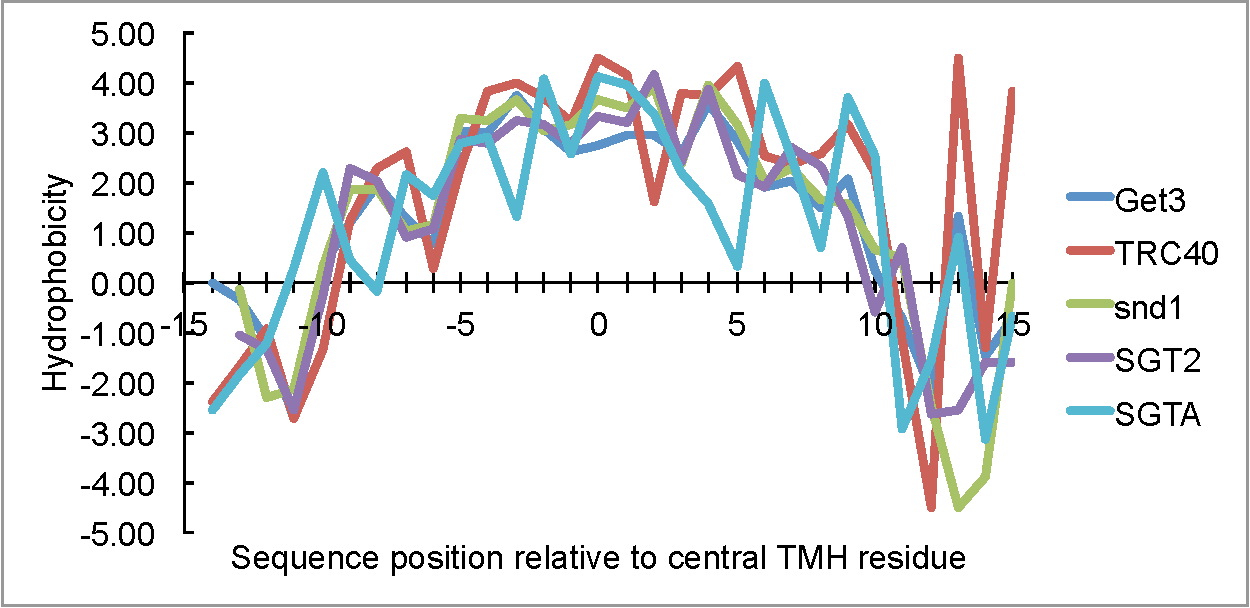
\includegraphics[width=1\textwidth]{TA_chapter/interaction-profile}
\captionof{figure}[The profile of TMH and flanks hydrophobicity from TA protein groups stratified by chaperone interactors.]
{\textbf{The profile of TMH and flanks hydrophobicity from TA protein groups stratified by chaperone interactors.}
On the horizontal axis is the position relative to the central TMH residue defined by UniProt.
On the vertical axis is the Kyte \& Doolittle hydrophobicity windowed across 5 residues allowing for half windows.
The chaperone interactors are colour coded according to the key.
}

\label{fig:interaction-profile}
\end{figure}

\subsection{Spontaneous Insertion May Be Achieved by Polar Strips in the TMH of Tail-Anchored Proteins}

The \gls{tmh} of cytochrome b5 and PTP1b are among the most hydrophobic of the \gls{ta} proteins and in theory misses the $\Delta$G requirements of a \gls{tmh} \cite{Rabu2008, Rabu2009}.
Indeed the \gls{tmh} is not trivial to predict and is not found in either dataset prepared herein.
Structural modelling and analysis thereof reveal features that may explain the ``missing hydrophobicity''~\cite{Hessa2005, Hedin2010, Hessa2007, Ojemalm2012} of these particular \gls{tmh}s.

The electrostatic surfaces are prototypical of a \gls{tmh} anchor with large ``positive\--inside'' patches \cite{VonHeijne1989, Andersson1992, Sharpe2010, Baeza-Delgado2013, Pogozheva2013, Baker2017} and a strong ``negative\--outside'' charge \cite{Baker2017}(Figure \ref{fig:cytb5-biochemistry}C).
Once in the membrane, this may allow it to be an effective anchor despite such poor hydrophobicity since it satisfies electrostatic coupling to the membrane potential.

Furthermore is the question of overcoming the unfavourable interaction most \gls{tmh}s would face when coming into contact with the highly polar membrane interface.
We observe a highly conserved strip of relatively polar / non-hydrophobic residues on one side of the \gls{tmh} core (in cytochrome b5 these are N112, P116, A120, A124 Y127, and R128).
Similarly, a polar face exists for the PTP1b \gls{tmh} (R430, N434, Y426, T422, and T419).
These polar faces would not be as repulsed by the interfacial environment as either a more hydrophobic \gls{tmh} or an equally hydrophobic \gls{tmh} with a different sequence and structure order (Figure \ref{fig:cytb5-biochemistry} and Figure \ref{fig:ptp1b-biochemistry}).
Scrambling the \gls{tmh} sequence whilst maintaining the same hydrophobicity reduces the insertion potential \cite{Brambillasca2006}; there is more to it than hydrophobicity alone.
It becomes apparent that the 3D arrangement of these relatively polar \gls{tmh} residues is conserved and is probably the key to spontaneous insertion of \gls{tmh}s.

\begin{figure}[!ht]
\centering
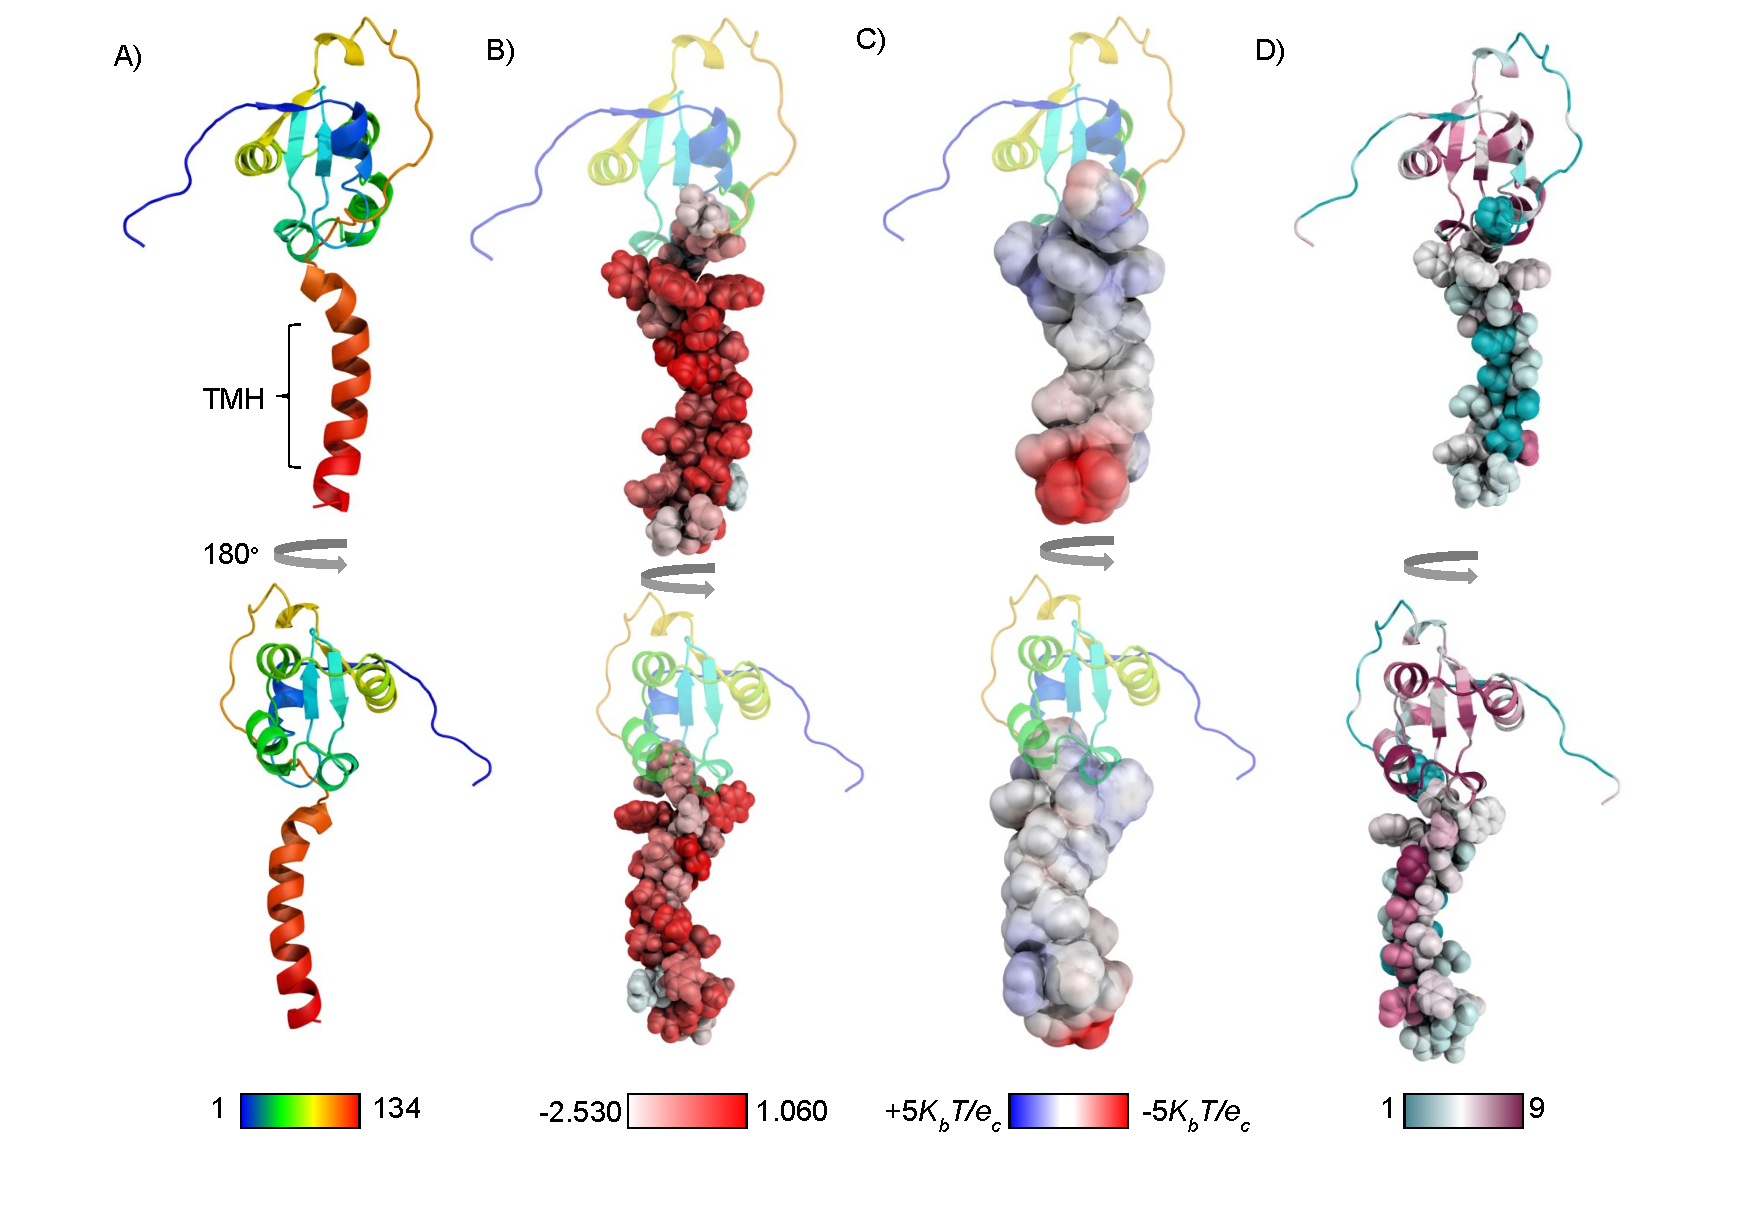
\includegraphics[width=1\textwidth]{TA_chapter/cytb5-biochemistry}
        \captionof{figure}[Structural biochemical analysis of a homology model of cytochrome b5.]{\textbf{Structural biochemical analysis of a homology model of cytochrome b5.}
        (A) The secondary structure of the protein coloured from the N terminus in blue to the C terminus in red coloured through the rainbow according to the residue number.
        (B) The hydrophobicity of the \gls{tmh} from white representing relatively polar residues to red showing relatively hydrophobic residues \cite{Eisenberg1984}.
        (C) The electrostatic surface with a threshold of $\pm5$ KT/e calculated by APBS in PyMol \cite{Baker2001}.
        Red patches are negatively charged whilst blue is positively charged.
        (D) The consurf scores on a scale of 1-9 (all residues had sufficient data) \cite{Ashkenazy2010}. Purple represents the most conserved whilst blue is the least.
        Note the correlation between the highly and modestly conserved \gls{tmh} residues and the relatively polar residues.
        Another observable feature is the very strong ``positive inside'' \cite{VonHeijne1989, Andersson1992, Sharpe2010, Baeza-Delgado2013, Pogozheva2013} and ``negative outside'' features which are associated with anchorage \cite{Baker2017}.
}

\label{fig:cytb5-biochemistry}
\end{figure}


\begin{figure}[!ht]
\centering
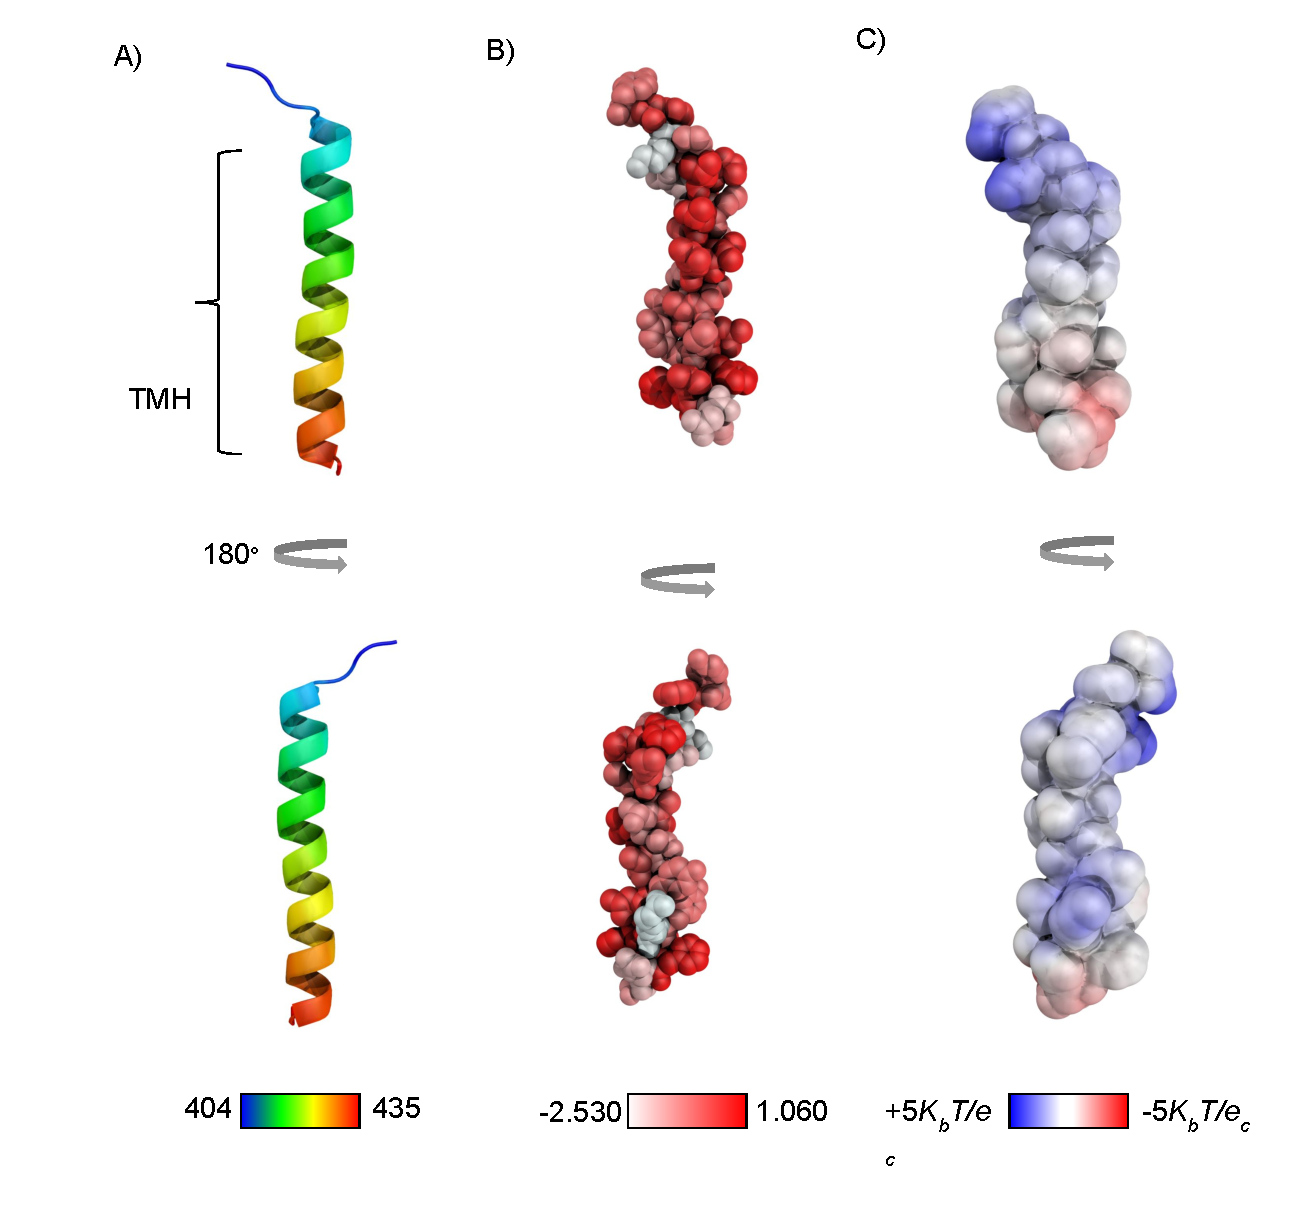
\includegraphics[width=1\textwidth]{TA_chapter/ptp1b-biochemistry}
        \captionof{figure}[Structural biochemical analysis of a homology model of PTP1b.]{\textbf{Structural biochemical analysis of a homology model of PTP1b.}
        (A) The secondary structure of the protein coloured from the N terminus in blue to the C terminus in red coloured through the rainbow according to the residue number.
        (B) The hydrophobicity of the \gls{tmh} from white representing relatively polar residues to red showing relatively hydrophobic residues \cite{Eisenberg1984}.
        (C) The electrostatic surface with a threshold of $\pm5$ KT/e calculated by APBS in PyMol \cite{Baker2001}.
        Red patches are negatively charged whilst blue is positively charged.
        Note the one hydrophobic face of the \gls{tmh} and the opposing relatively polar face.
        Another observable feature is the ``positive inside'' \cite{VonHeijne1989, Andersson1992, Sharpe2010, Baeza-Delgado2013, Pogozheva2013} and ``negative outside'' features which are associated with anchorage \cite{Baker2017}.
}

\label{fig:ptp1b-biochemistry}
\end{figure}

\section{Summary}

Here, we have observed a large biochemical distinction between \gls{ta} proteins with different terminal destinations.
Previously it was known that both hydrophobicity and charge are involved in targeting \cite{Costello2017}.
In this study, we find that the location of the charge along and around the \gls{tmh} is different in different subcellular compartments.
Crucially, there is a shift in the charged residue inside\--outside tandem in the \gls{tmh} flanking residues in different organelles which in mitochondria goes against the membrane\--potential electrostatic coupling.
Furthermore, the missing hydrophobicity of mitochondrial \gls{ta} proteins can be in part attributed to the high abundance of alanine rather than leucine or isoleucine in the \gls{tmh}.
We expected to see evolutionary adaptations of \gls{tmh} hydrophobicity to species-specific membranes, even within eukaryotes~\cite{Baker2017, Sharpe2010}.
In this study using both a manually curated dataset from UniProt and an automatically filtered list using SwissProt annotation, we do not observe any strong differences.
Since we could not scrutinise a difference in the species, the strong hydrophobic differences between organelle \gls{tmh}s are indicative of a stronger adaptation pressure than between species.
These differences are likely to be partially adaptations to the organelle location membrane type and also possible cryptic biological factors that play a role in their targeting via chaperone\--binding affinity.
This could be a functional similarity to the signal-anchored proteins.
Signal anchored proteins contain a single hydrophobic segment that serves as both a mitochondrial targeting signal and a membrane anchor.
Signal anchored proteins, along with some \gls{ta} proteins, have been shown to be able to spontaneously insert into the membrane independently from the translocon~\cite{Elisa2012, Lan2000, Colombo2009}.

We could not find any clear trends or perform statistical work on the interactor datasets due to the small sample sizes, however, as the databases are enriched, this same method will be able to answer the questions about chaperone affinity with more accuracy in the future.

Furthermore, the spontaneously inserting \gls{ta} proteins PTP1b and cytochrome b5 appear to share a polar face that emerges in structural models and a strong positive\--inside negative\--outside electrostatic surface.
The polar face may be responsible for the promotion insertion potential in the absence of insertion proteins since when the sequence is scrambled, the insertion potential is reduced \cite{Brambillasca2006}.
The positively and negatively charged residues are distributed like an ideal anchoring \gls{tmh} \cite{Baker2017} which could allow the marginally hydrophobic \gls{tmh} to perform as a suitable membrane anchoring feature.
